\documentclass[11pt]{article}
\usepackage[T1]{fontenc}
\usepackage{amssymb}
\usepackage{amsmath}
\usepackage{amsthm}
\usepackage{bm}
\usepackage{graphicx}
\usepackage{dsfont}
\usepackage[makeroom]{cancel}
\usepackage{mathtools}
\usepackage{commath}
\usepackage[english]{babel}
\usepackage[utf8]{inputenc}
\usepackage{fancyhdr}
\usepackage{bold-extra}
\usepackage{color}   
\usepackage{hyperref}
\usepackage{tocloft}
\usepackage[shortlabels]{enumitem}
\usepackage{pgfplots}
\usepgfplotslibrary{fillbetween}
\usetikzlibrary{patterns}
\usepackage{listings}
\usepackage{multicol}

\definecolor{dkgreen}{rgb}{0,0.6,0}
\definecolor{gray}{rgb}{0.5,0.5,0.5}
\definecolor{mauve}{rgb}{0.58,0,0.82}

\lstset{frame=tb,
  language=C++,
  aboveskip=3mm,
  belowskip=3mm,
  showstringspaces=false,
  columns=flexible,
  basicstyle={\ttfamily},
  numbers=none,
  numberstyle=\tiny\color{gray},
  keywordstyle=\color{blue},
  commentstyle=\color{dkgreen},
  stringstyle=\color{mauve},
  breaklines=true,
  breakatwhitespace=true,
  tabsize=2
}

\theoremstyle{definition}
\newtheorem*{thm*}{Theorem}
\newtheorem{thm}{Theorem}[section]

\newtheorem{defn}[thm]{Definition}
\newtheorem{exmp}[thm]{Example}
\newtheorem{prop}[thm]{Proposition}
\newtheorem{cor}[thm]{Corollary}
\newtheorem{lemma}[thm]{Lemma}
\newtheorem{remark}[thm]{Remark}
\newtheorem{notation}[thm]{Notation}
\newtheorem{exercise}[thm]{Exercise}
\newtheorem{app}[thm]{Applications}
\newtheorem{none}[thm]{}
\newtheorem{idea}[thm]{Idea}

\newcommand{\N}{\ensuremath{\mathbb{N}}}
\newcommand{\Z}{\ensuremath{\mathbb{Z}}}
\newcommand{\Q}{\ensuremath{\mathbb{Q}}}
\newcommand{\R}{\ensuremath{\mathbb{R}}}
\newcommand{\C}{\ensuremath{\mathbb{C}}}

\newcommand\bigLozenge{\mathop{\mathpalette\bigL@zenge\relax}}
\newcommand\bigL@zenge[2]{%
  \vcenter{\hbox{\m@th
    \scalebox{\ifx#1\displaystyle 2\else1.2\fi}{$#1\blacklozenge$}%
  }}%
}
\makeatother

% L'Hopital's Rule
\newcommand{\lhr}{\stackrel{\mathclap{\mbox{\normalfont\tiny L'HR}}}{=}}

% 1-inch margins
\topmargin 0pt
\advance \topmargin by -\headheight
\advance \topmargin by -\headsep
\textheight 8.9in
\oddsidemargin 0pt
\evensidemargin \oddsidemargin
\marginparwidth 0.5in
\textwidth 6.5in

\parindent 0in
\parskip 1.5ex

% hyperlinks
\hypersetup{
  colorlinks=true, 
  linktoc=all,     % table of contents is clickable  
  allcolors=blue   % all hyperlink colours
}

% table of contents
\addto\captionsenglish{
  \renewcommand{\contentsname}%
    {Table of Contents}%
}

\fancypagestyle{plain}{%
\fancyhf{} % clear all header and footer fields
\lhead{CS 246: Object-Oriented Software Development}
\fancyhead[R]{Table of Contents}
%\headrule
\fancyfoot[C]{\thepage} % except the center
%\renewcommand{\headrulewidth}{0pt}
%\renewcommand{\footrulewidth}{0pt}
}

% headers and footers
\pagestyle{fancy}
\renewcommand{\sectionmark}[1]{\markboth{#1}{#1}}
%\lhead{Winter 2019}
\lhead{CS 246: Object-Oriented Software Development}
\fancyhead[R]{Chapter \thesection: \em \leftmark}
\cfoot{\thepage}
\setlength\headheight{14pt}

% title and preface formatting
\newcommand{\newtitle}[4]{
  \begin{center}
	\huge{\textbf{\textsc{#1 Course Notes}}}
    
	\large{\sc #2}
    
	{\sc #3 \textbullet\, #4 \textbullet\, University of Waterloo}
	\normalsize\vspace{1cm}\hrule\vspace{0.5cm}
	
	%\textbf{Preface}
  \end{center}
  %\vspace{-0.4cm}
  %These notes were created as a resource for personal use, and for current, past, and future students of the course. They may contain errors and inconsistencies. If you notice any errors or have other inquiries regarding these notes, feel free to e-mail me at {\tt mltlee@uwaterloo.ca}. \vspace{1cm}\hrule\vspace{0.5cm}
}

% \setcounter{section}{-1}

\pgfplotsset{compat=1.15}

% new proof environment
\makeatletter
\newenvironment{pf}[1][\proofname]{\par
  \pushQED{\qed}%
  \normalfont \topsep0\p@\relax
  \trivlist
  \item[\hskip\labelsep\itshape
  #1\@addpunct{.}]\ignorespaces
}{%
  \popQED\endtrivlist\@endpefalse
}
\makeatother

\begin{document}

% title and preface

\newtitle{CS 246}{Object-Oriented Software Development}{Brad Lushman}{Fall 2019}

\rhead{Table of Contents}

\tableofcontents
\vspace{1cm}\hrule
\clearpage
\fancyhead[R]{Lecture \thesection: \leftmark}

\section{September 5, 2019}

{\bf Grading:} Assignments: 40\% (5\%, 7\%, 7\%, 9\%, 12\%), Midterm: 20\%, Final: 40\% 

{\bf Modules:} Linux Shell, C++, Tools, Software Engineering

\subsection{Linux Shell}
Shell: \vspace{-0.25cm}
\begin{itemize}
    \item interface to the OS - gets OS to run programs, manage files, etc.
    \item graphical (click/touch)
    \item command line - type commands at a prompt, more versatile
\end{itemize}
\vspace{-0.25cm} 
This course uses bash, a command line shell.

To check this, login and type {\tt echo \$0}.

{\tt cat} -- displays the contents of a file (e.g. {\tt cat /usr/share/dict/words}) \vspace{-0.25cm}
\begin{itemize}
    \item first {\tt /} is called the root (top) directory
    \item {\tt usr}, {\tt share}, {\tt dict} are directories
    \item {\tt words} is the file
\end{itemize}
\vspace{-0.25cm}
In Linux, a directory is a special kind of file.

In Linux, every line of a valid text file must end with a newline character, {\bf including the last one}. Marmoset checks for this.

Use {\tt \^ \null C} (Ctrl + C) to stop.

{\tt ls} -- list files in current directory (non-hidden files)

{\tt ls -a} -- list all files (including hidden ones - name begins with {\tt .})

{\tt pwd} -- prints the current directory

{\tt wc} -- shows the number of lines, words, and characters in a file

\subsection{Output and Input Redirection}
Typing {\tt cat} on its own makes it wait and prints out everything you type onto the screen. 

This can be useful if we can capture the output in a file.

To do this, we can use {\tt cat > myfile.txt}.

To stop, use {\tt \^ \null D} at the beginning of a line. This sends an end-of-file (EOF) signal to {\tt cat}.

In general, using {\tt command args > file} executes {\tt command args} and captures the output in {\tt file} instead of the screen. This is called {\bf output redirection}.

We can also redirect input. Consider {\tt cat < file}. \vspace{-0.25cm}
\begin{itemize}
    \item input comes from {\tt file} instead of the keyboard
    \item displays content of {\tt file}
    \item seems equivalent to {\tt cat file}
\end{itemize}
\vspace{-0.25cm}
The difference between the two (important):

{\tt cat file}  \vspace{-0.25cm}
\begin{itemize}
    \item passes the name {\tt file} as an {\bf argument} to {\tt cat}
    \item {\tt cat} opens the file and displays its contents
\end{itemize}
\vspace{-0.25cm}

{\tt cat < file} \vspace{-0.25cm}
\begin{itemize}
    \item {\bf the shell} opens {\tt file} and passes its contents to {\tt cat} in place of keyboard input
\end{itemize}
\vspace{-0.25cm}
Both input and output redirection can be done: {\tt cat < infile > outfile}. \vspace{-0.25cm}
\begin{itemize}
    \item takes characters from {\tt infile} and sends them to {\tt outfile}
    \item copies the file
\end{itemize}

\subsection{Globbing Patterns}
{\tt *.txt} is called a globbing pattern. {\tt *} means to match any sequence of characters. The shell finds all files in the current directory whose names match the pattern and substitutes them on the command line. 

For example, {\tt cat *.txt} transforms into {\tt cat a.txt b.txt c.txt}. {\tt cat} opens all three and displays them.

More globbing patterns can be found on the Linux sheet.

\subsection{Streams}
Every process is attached to 3 {\bf streams}.

{\tt stdin} is the input, and {\tt stdout} and {\tt stderr} are the outputs.

By default, {\tt stdin} is the keyboard, and {\tt stdout} and {\tt stderr} are on the screen.

Redirection: {\tt <} connects {\tt stdin} to a file, {\tt >} connects {\tt stdout} to a file, and {\tt 2>} connects {\tt stderr} to a file. 

{\tt stderr} is a separate output stream for error messages. We can send output and error messages to different places, and error messages don't corrupt the format of output files.

Also, {\tt stdout} may be {\bf buffered}. The system may wait to accumulate output before actually displaying (flushing) it. {\tt stderr} is never buffered -- error messages are received immediately.

\subsection{Pipes} 
{\tt |} -- use output of one program as input to another, and sets second program's {\tt stdin} to first programs {\tt stdout}.

{\bf Example.} How many words occur in the first 20 lines of {\tt myfile.txt}?

{\tt head -n file} gives the first {\tt n} lines of {\tt file}.

{\tt wc -w} gives the number of words.

Hence we can pipe the former into the latter with {\tt head -20 myfile.txt | wc -w}.

We can also use {\tt cat myfile.txt | head -20 | wc -w}.

{\bf Example.} Suppose {\tt words1.txt}, {\tt words2.txt}, etc. contains lists of words, one per line. Produce a duplicate-free list of all words that occur in any of these files.

{\tt uniq} -- removes {\em adjacent} duplicate entries

{\tt sort} -- sorts the lines of a file

Solution: {\tt cat words*.txt | sort | uniq}

{\bf Example.} Print the 10 most frequent words in a file and their frequency.

Solution: {\tt sort myfile | uniq -c | sort -n | tail -10}, if each word is on a different line

{\tt tr ' ' '\symbol{92}n' myfile | sort | uniq -c | sort -n | tail -10} otherwise
\newpage
\section{September 10, 2019}
\subsection{Embedded Commands}
Consider {\tt echo "Today is \$(date) and I am \$(whoami)"}. 

The shell executes {\tt date} and {\tt whoami}, and substitutes the result into the second line.

Note that using {\tt echo Today is \$(date) and I am \$(whoami)}, with no quotes, takes everything as separate arguments.

Inside single quotes, such as {\tt echo 'Today is \$(date) and I am \$(whoami)'}, results in no {\tt \$}-expansion.

Using {\tt echo *} returns all the files.

Both single and double quotes will suppress glob expansion. For example, {\tt echo "*"} returns {\tt *}.

\subsection{Pattern-Matching in Text Files}
{\tt grep/egrep} -- (extended) global regular expression print

{\tt egrep pattern file} prints every line in {\tt file} that contains {\tt pattern}.

{\bf Example.} Print every line in {\tt myfile} that contains {\tt cs246}.

Solution: {\tt egrep cs246 myfile}

{\bf Example.} How many lines in {\tt myfile} contain {\tt cs246} or {\tt CS246}?

Solutions: 
{\tt egrep "cs246|CS246" myfile | wc -l} or {\tt egrep "(cs|CS)246" myfile | wc -l}

{\tt (c|C)(s|S)246} or {\tt [cC][sS]246} will also match {\tt cS246} and {\tt Cs246}. 

{\tt [...]} means any one character between {\tt [} and {\tt ]}.

{\tt [\^ \null ...]} means any one character {\it except} {\tt ...}.

The available patterns are called {\bf regular expressions} (different from globbing patterns). 

We can also add an optional space with {\tt [cC][sS] ?246}. 

{\tt ?} matches 0 or 1 of the preceding pattern (in this case, 0 or 1 spaces).

{\tt *} matches 0 or more of the preceding pattern. For example, {\tt (cs)*246} will match {\tt 246}, {\tt cs246}, {\tt cscs246}, etc.

{\tt +} means 1 or more of the preceding pattern.

{\tt .} matches any single character.

{\tt .*} matches anything. {\tt egrep "cs.*246" myfile} would match any lines containing {\tt cs...(anything)...246}.

{\tt \^\null.\$} means the beginning or end of line. {\tt \^\null cs246} matches lines that start with {\tt cs246}, and {\tt \^\null cs246\$} matches lines exactly equal to {\tt cs246}.

{\bf Example.} Print all lines of even length.

Solution: {\tt \^\null(..)*\$}

{\bf Example.} Print all files in the current directory whose names contain exactly one {\tt a}.

Solution: {\tt ls | egrep "\^\null[\^\null a]*a[\^\null a]*\$}"

{\bf Example.} Find all words in the global dictionary that start with {\tt e} and have 5 characters.

Solution: {\tt egrep "\^\null e....\$" /usr/share/dict/words}

\subsection{Permissions}
{\tt ls -l} -- long form listing

Suppose we have a line {\tt -rw-r--------- 1 j2smith j2smith 25 Sep 9 15:27 abc.txt}.

The first character, {\tt -}, is the type. This can be {\tt -}, an ordinary file, or {\tt d}, a directory. \\
The following three characters, {\tt rw-}, is the (owner) user permissions. \\
The next three characters after that, {\tt r-\null-} is group permissions. \\
The last three characters, {\tt -\null-\null-}, are other permissions. \\
The next number, {\tt 1}, is the number of links. \\
After that, {\tt j2smith}, is the owner. \\
Then, {\tt j2smith}, is the groups. \\
The number after that, {\tt 25}, is the size. \\
Next, {\tt Sep 9 15:27} is the last modified date. \\
Finally, {\tt abc.txt} is the name of the file.

\subsection{Groups}
A user can belong to one or more groups, and a file can be associated with one group.

User bits apply to the file's owner.

Group bits apply to members of the file's group (other than the owner).

Other bits apply to everyone else.

{\tt r} is the read bit, {\tt w} is the write bit, and {\tt x} is the execute bit.

\begin{table}[h]
\begin{tabular}{l|l|l}
Bit     & Meaning for ordinary files        & Meaning for directories        \\ \hline
{\tt r} & file's contents can be read       & \begin{tabular}[c]{@{}l@{}}directory's contents can be read \\ (e.g. {\tt ls}, globbing, tab completion)\end{tabular} \\ \hline
{\tt w} & file's contents can be modified   & \begin{tabular}[c]{@{}l@{}}directory's contents can be modified\\ (can add/remove files)\end{tabular} \\ \hline
{\tt x} & file can be executed as a program & \begin{tabular}[c]{@{}l@{}}directory can be navigated\\ (i.e. can {\tt cd} into the directory)\end{tabular}
\end{tabular}
\end{table}

If the directory's {\tt x} bit is not set, then there is no access at all, nor to any file/directory within it.

{\tt chmod mode file} -- change permissions

{\tt mode: usertypes operator perms}

{\tt usertypes:} {\tt u} (user), {\tt g} (group), {\tt o} (other), {\tt a} (all)

{\tt operator:} {\tt +} (add person), {\tt -} (remove person), {\tt =} (set perms exactly)

{\tt perms:} {\tt r}, {\tt w}, {\tt x}

{\bf Example.} Give others read permission.

Solution: {\tt chmod otr file}

{\bf Example.} Make everyone's permission {\tt rx}.

Solution: {\tt a=rx}

{\bf Example.} Give the owner full control.

Solution: {\tt u+rwx} (or {\tt u=rwx})
\newpage
\section{September 12, 2019}
\subsection{Shell Scripts}
A shell script is a file containing sequences of shell commands, executed as a program. 

{\bf Example.} Print the date, current user, and current directory.

{\tt myscript} contains

\begin{verbatim}
#!/bin/bash
date
whoami
pwd
\end{verbatim}

{\tt \#!/bin/bash} is called the "shebang line", and says to execute this file as a bash script.

First, give the file execute permission with {\tt chmod u+x myscript}.

Then run the file with {\tt ./myscript}.

To debug a script, use {\tt bash -x myscript}, or add {\tt -x} to the shebang line.

\subsection{Variables}
We can assign a variable with {\tt x=1} (no spaces). 

Use {\tt \$} when fetching the value of a variable.

No {\tt \$} is used when setting a variable.

For good practice, use {\tt \$\{x\}}.

To remove suffixes, {\tt \$\{A\%foo\}} removes {\tt foo} from the end of {\tt A} (this does not change the variable itself, just the output).

All variables contain {\bf strings}. Here, {\tt \$x} is the {\bf string} 1, not the number.

You can test with {\tt [} and {\tt ]}. For example, {\tt [ "hi" = "hi" ]}, or {\tt [ "\$A" -le "\$B" ]}.

{\bf Example.} Consider {\tt dir=\~\null/cs246}. 

{\tt echo \$\{dir\}} returns {\tt /u/userid/cs246}.

{\tt ls \$\{dir\}} returns the contents of the above directory.

There are some "global" variables.

Important: {\tt PATH} is a list of directories. When you type a command, the shell searches these directories, in order, for a program with that name. 

{\tt echo "\$PATH"} returns the path, while {\tt echo '\$PATH'} returns {\tt \$PATH}. {\tt \$}-expansion is only in double quotes.

There are special variables for scripts: {\tt \$1}, {\tt \$2}, etc. -- command line args. 

{\bf Example.} Check whether a word is in the dictionary.

Solution: {\tt ./isItAWord hello} where {\tt isItAWord} contains 
\begin{verbatim}
#!/bin/bash
egrep "^$1$" /usr/share/dict/words
\end{verbatim}
This prints nothing if the word is not found, and prints the word if found.

{\bf Example.} A good password is not in the dictionary. Determine if the password is good.

Solution: First consider 
\begin{verbatim}
#!/bin/bash
egrep "^$1$" /usr/share/dict/words > /dev/null
\end{verbatim}

(Useful: {\tt /dev/null} suppresses output.)

Every program returns a status code when finished.

In Linux, {\tt 0} is success, {\tt 1} is failure. For example, {\tt egrep} returns {\tt 0} if found, {\tt 1} if not found.

{\tt \$?} is the status of the most recently executed command.

Script continued:
\begin{verbatim}
if [ $? -eq 0 ]; then 
  echo Bad password 
else 
  echo Maybe a good password 
fi
\end{verbatim}

Alternatively, we can replace the first line with

\begin{verbatim} 
if egrep ... > /dev/null ; then
\end{verbatim}

To verify that the correct number of arguments are there, print an error message if wrong.
\begin{verbatim}
#!/bin/bash
usage() {
  echo "usage: $0 password" 1>&2
}
if [ $# -ne 1 ]; then
  usage
  exit 1
fi
(as before)
\end{verbatim}
{\tt \$0} is the name of the program/script, and {\tt 1>\&2} redirects {\tt stdout} to {\tt stderr}. {\tt \$\#} is the number of arguments. 

\subsection{Loops}
{\bf Example.} Print all numbers from 1 to {\tt \$1}. 

Solution: 
\begin{verbatim}
#!/bin/bash
x=1
while [ $x -le $1 ]; do
  echo $x
  x=$((x+1))
done
\end{verbatim}

Use {\tt \$((...))} for arithmetic.

A simple {\tt for} loop
\begin{verbatim}
for x in a b c; do
  echo $x
done
\end{verbatim}
would return
\begin{verbatim}
a
b
c
\end{verbatim}

\subsection{Applications of Shell Scripts}
{\bf Example.} Looping over a list: rename all {\tt .cpp} files to {\tt .cc}.

Solution:
\begin{verbatim} 
for name in *.cpp; do
  mv ${name} ${name%cpp}cc
done
\end{verbatim}

{\tt name\%cpp} is the value of {\tt name}, without the trailing {\tt cpp}.

{\bf Example.} How many lines does word {\tt \$1} occur in file {\tt \$2}?

Solution:
\begin{verbatim}
for word in $(cat "$2"); do
  if [ $word = "$1" ]; then
    x=$((x+1))
  fi
done
echo $x
\end{verbatim}

{\bf Example.} Payday is the last Friday of the month. When is this month's payday?

Solution: We have two tasks: compute payday, and report the answer.

The command {\tt cal} returns the calendar for the current month. Then, the line
\begin{verbatim}
cal | awk '{print $6}'
\end{verbatim}
returns
\begin{verbatim}
Fr
6
13
20
27
\end{verbatim}
Then 
\begin{verbatim}
cal | awk '{print $6}' | egrep "[0-9]"
\end{verbatim}
gives
\begin{verbatim}
6
13
20
27
\end{verbatim}
and taking the tail with 
\begin{verbatim}
cal | awk '{print $6}' | egrep "[0-9]" | tail -1
\end{verbatim}
we get
\begin{verbatim}
27
\end{verbatim}
Then our script would be
\begin{verbatim}
report() {
  if [ $1 -eq 31 ]; then
    echo "This month: the 31st"
  else
    echo "This month: the ${1}th"
  fi
}
report $(cal | awk '{print $6}' | egrep "[0-9]" | tail -1)
\end{verbatim}
Generalizing to any month, note that
\begin{verbatim}
cal October 2019
\end{verbatim}
gives that month's calendar. We can replace the last line of the above script with 
\begin{verbatim}
report $(cal $1 $2 | awk '{print $6}' | egrep "[0-9]" | tail -1) $1
\end{verbatim}
Note that {\tt \$1} and {\tt \$2} are blank if not supplied, hence reverting to previous behaviour. Here, the month name, {\tt \$1} is the second argument. Below, {\tt \$2} is the second argument.
\begin{verbatim}
report() {
  if [ $2 ];
    echo -n $2
  else
    echo -n "This month"
  fi
  if [ $1 -eq 31 ]; then
    echo ": the 31st"
  else
    echo ": the ${1}th"
  fi
}
\end{verbatim}

{\bf Example.} Write a script called {\tt mean}. It takes {\tt filename} as an argument, computes the mean of the numbers in that file, and prints it to {\tt stdout}.

Solution:
\begin{verbatim}
#!/bin/bash
if [ $# -ne 1 ], then
  echo "$0 requires exactly one argument"
  exit 1
fi
A="0" # sum of all numbers
B="0" # number of numbers
for n in $(cat $1); do
  A=$(($A + $n))
  B=$(($B + 1))
done
echo $(($A / $B))
\end{verbatim}
\newpage
\section{September 17, 2019}

\subsection{Testing}
Testing is an essential part of program development. It begins {\it before} you start coding (i.e. creating test suites for expected behaviour) and continues while you are coding. It is not the same as debugging -- you cannot debug without testing first. Ideally, the programmer is not the tester (there is no psychological barrier). 

{\bf Human Testing:} Humans look for flaws (i.e. code inspections). Humans cannot check everything.

{\bf Machine Testing:} Runs program on selected inputs and compares with expected outputs. Again, this cannot check everything, and test cases must be chosen carefully. 

{\bf Black/White/Grey Box Testing:} No/full/some knowledge of program input. 

Start with black box testing, and then supplement with white box. 

Some tips: \vspace{-0.25cm}
\begin{itemize}
    \item Test various classes of input (e.g. numeric ranges, positive versus negative).
    \item Test boundaries of valid ranges (edge cases). 
    \item Test multiple simultaneous boundaries (corner cases).
    \item Use intuition and experience to guess at likely errors.
    \item Test extreme cases (within reason).
\end{itemize}
\vspace{-0.25cm}
When white box testing, execute all logical paths through the program, and make sure every function is called.

{\bf Do not test invalid input, unless a behaviour has been prescribed.} If the input is invalid, there is no corresponding correct output, so any such test case would be meaningless.

{\bf Regression Testing:} Ensures that new changes to program don't break the old test cases (test suites, testing scripts).

\subsection{C++}

Hello world in C++:
\begin{lstlisting}
#include <iostream>
using namespace std;
int main() {
    cout << "Hello world" << endl;
    return 0;
}
\end{lstlisting}
Notes: \vspace{-0.25cm}
\begin{itemize}

    \item {\tt void main() ...} is illegal in C++, unlike C
    
    \item {\tt stdio.h}, {\tt printf} are still available in C++ (but banned in this course)
    
    \item preferred C++ I/O {\tt <iostream>}
    
    {\tt std::cout <\null< \_\_\_ <\null< \_\_\_ <\null< \_\_\_ ...} where each {\tt \_\_\_} is data
    
    {\tt std::endl} means the end of line
    
    \item {\tt using namespace std} lets you omit the {\tt std::} prefix
    
    \item {\tt return} statement can be omitted from {\tt main} ({\tt 0} assumed)
    
    \item {\tt \$?} returns the status code
    
\end{itemize}
\vspace{-0.25cm}
Compiling a C++ program: {\tt g++ -std=c++14 -Wall program.cc -o program}

{\tt -std=c++14} is the current version, {\tt -Wall} means to warn all, {\tt program.cc} is the name of the program, and {\tt -o program} is the name of the output file (if not given, {\tt a.out}). 

Alternatively: {\tt g++14 program.cc -o program}

Most C programs are valid C++ -- there will be no C review in this course. 

\subsection{Input/Output}
There are 3 I/O streams: 

{\tt cout/cerr} -- for printing to {\tt stdout/stderr} \\
{\tt cin} -- for reading from {\tt stdin} 

I/O operators: 

{\tt <\null<} -- "put to" (output) \\
{\tt >\null>} -- "get from" (input)

To remember this, the operator "points" in the direction of information flow.

{\bf Example.} Add two numbers.

Solution:
\begin{lstlisting}
#include <iostream>
using namespace std;
int main() {
    int x, y;
    cin >> x >> y;
    cout << x + y << endl;
}
\end{lstlisting}
We will omit the first two lines from now on (assume that they are always there). 

Note: {\tt cin >\null>} ignores whitespace (space, tab, newline). 

If the number is too big, the program will return the largest number possible.

If the input is exhausted before we get 2 integers, then the statement fails. 

If the read failed, {\tt cin.fail()} will be true.

If {\tt EOF}, {\tt cin.eof()} and {\tt cin.fail()} are both true, but not until the attempted read fails.

{\bf Example.} Read all integers from {\tt stdin} and {\tt echo} them, one per line, to {\tt stdout}. Stop on bad input or {\tt EOF}. 

Solution:
\begin{lstlisting}
int main() {
    int i;
    while(true) {
        cin >> i;
        if(cin.fail()) break;
        cout << i << endl;
    }
}
\end{lstlisting}
Note: There is an implicit conversion from {\tt cin} to {\tt bool} (true if success, false if failure). This lets {\tt cin} be used as a condition.

Using this, we can rework the previous solution:
\begin{lstlisting}
int main() {
    int i;
    while(true) {
        cin >> i;
        if(!cin) break;
        cout << i << endl;
    }
}
\end{lstlisting}
Note: In C, {\tt >\null>} is the right bitshift operator. {\tt a >\null> b} shifts {\tt a}'s bits to the right by {\tt b} spots. 

For example, consider {\tt 21 >\null> 3}: \\
$21 = 10101_2$, removing last 3 digits, {\tt 21 >\null> 3} returns $10_2 = 2$

Essentially, it computes $a / 2^b$.

This is the same in C++. But when the left hand side is {\tt cin}, {\tt >\null>} is the "get from" operator. 

The operator {\tt >\null>} inputs {\tt cin} (istream) and some data (varying types), and outputs {\tt cin} back (istream).

From the previous example, another solution is
\begin{lstlisting}
int main() {
    int i;
    while(true) {
        if(!(cin >> i)) break;
        cout << i << endl;
    }
}
\end{lstlisting}
We can also write
\begin{lstlisting}
int main() {
    int i;
    while(cin >> i) {
        cout << i << endl;
    }
}
\end{lstlisting}

{\bf Example.} Read all integers and {\tt echo} to {\tt stdout} until {\tt EOF}. Skip non-integer input.

Solution:
\begin{lstlisting}
int main() {
    int i;
    while(true) {
        if(!(cin >> i)) {
            if(cin.eof()) break; // EOF - done
            cin.clear(); // cin stops working until cleared
            cin.ignore(); // ignore next character
        } else cout << i << endl;
    }
}
\end{lstlisting}
\newpage
\section{September 19, 2019}

\subsection{I/O Manipulators}
Consider printing a number in hexadecimal.
\begin{lstlisting}
cout << hex << 95 << endl; // prints 5f
\end{lstlisting}
{\tt hex} is an I/O manipulator. It says to print all subsequent ints in hexadecimal. 

To go back to decimal, use
\begin{lstlisting}
cout << dec;
\end{lstlisting}
There are other manipulators as well (see C++ reference {\tt <iomanip>}).

\subsection{Strings}
Recall that in C, a string is an array of characters ({\tt char*} or {\tt char[]}) terminated by {\tt \textbackslash0}.
You must explicitly manage memory, allocating more memory as strings get larger. It is easy to overwrite {\tt \textbackslash0} and corrupt memory.

In C++, it is comparatively easier to use strings. Use {\tt \#include <string>}. It grows as needed and is safer to manipulate. 

{\bf Example.} {\tt string s = {\color{mauve} "Hello"};}

{\tt {\color{mauve} "Hello"}} is a C-style string (char array). {\tt s} is a C++ string created from a C string on initialization.

\subsubsection*{String Operations}

{\bf Equality/inequality:} {\tt s1 == s2}, {\tt s1 != s2}

{\bf Comparison:} {\tt s1 <= s2} (lexicographic)

{\bf Length:} {\tt s.length()}

{\bf Get individual characters:} {\tt s[0]}, {\tt s[1]}, etc.

{\bf Concatenation:} {\tt s3 = s1 + s2}, {\tt s3 += s4}

{\bf Example.} A program to read in and print a string:
\begin{lstlisting}
int main() {
    string s;
    cin >> s; 
    cout << s << endl;
}
\end{lstlisting}
This reads a string, skips leading whitespace, and stops at whitespace (i.e. reads one word). 

If we want the whitespace, we can use {\tt getline(cin, s)}. This reads from the current position to next newline into {\tt s}. 

\subsection{Stream Abstraction}
Stream abstraction applies to other sources of data.

\subsubsection*{Files}

Read from a file instead of {\tt stdin}. \\
{\tt std::ifstream} reads from a file. \\
{\tt std::ofstream} writes to a file.

File access in C:
\begin{lstlisting}
#include <stdio.h>
int main() {
    char s[256];
    FILE *f = fopen("file.txt", "r"); // r means open for reading
    while(true) {
        fscanf(f, "%255s", s);
        if(feof(f)) break;
        printf("%s\n", s);
    }
    fclose(f); // give file access back to OS
}
\end{lstlisting}

File access in C++:
\begin{lstlisting}
#include <iostream>
#include <fstream>
#include <string>
using namespace std;
int main() {
    ifstream f {"file.txt"}; // declaring and initializing an ifstream opens the file
    string s;
    while(f >> s) {
        cout << s << endl;
    } // file is closed when the ifstream (f) goes out of scope
}
\end{lstlisting}
Anything you can do with {\tt cin/cout}, you can do with an {\tt ifstream/ofstream}.

For example, for a string, attach a stream to the string variable and read from or write to the string.
\begin{lstlisting}
string intToString(int n) {
    ostringstream sock;
    sock << n;
    return sock.str();
}
\end{lstlisting}

{\bf Example.} Convert a string to a number.

Solution:
\begin{lstlisting}
int main() {
    int n;
    cout << "Hello, " << endl;
    while(true) {
        cout << "enter a number." << endl;
        cin >> s;
        istringstream sock{s};
        if(sock >> n) break;
        cout << "I said, ";
    }
    cout << "You entered " << n << endl;
}
\end{lstlisting}

{\bf Example.} Revisited: {\tt echo} all numbers and skip all non-numbers.

Solution:
\begin{lstlisting}
int main() {
    string s;
    while(cin >> s) { // only way to fail is EOF
        istringstream sock{s};
        int n;
        if(sock >> n) cout << n << endl;
    }
}
\end{lstlisting}
Differences between the two solutions: this one will take the first number and throw the rest away, while the previous one will take all numbers inside. (e.g. {\tt 123abc456} gives only {\tt 123} for the above, while for the previous it would return {\tt 123} and {\tt 456}.)

For the above two examples, there is no need to reset because it is a new sock each time.

\subsection{Default Value in Parameters}
Consider the following:
\begin{lstlisting}
void printSuiteFile(string name = "suite.txt") {
    ifstream f{name};
    string s;
    while(f >> s) cout << s << endl;
}
\end{lstlisting}
Calling {\tt printSuiteFile();} prints from {\tt suite.txt} by default.

Note: parameters with defaults must be last.

\subsection{Overloading}
In C++, functions with different parameter lists can share the same name. 

For example, to negate both integers and booleans, we can write
\begin{lstlisting}
int neg(int a) { return -a; }
bool neg(bool b) { return !b; }
\end{lstlisting}
This is known as {\bf overloading}. The correct version of {\tt neg}, for each function call, is chosen {\it by the compiler} (i.e. at compile time). It is based on the number and the types of the arguments; just differing in the return type is not enough.

The operators {\tt >\null>} and {\tt <\null<} are overloaded -- the behaviour depends on the types of arguments.

\subsection{Structs}
Consider the following struct:
\begin{lstlisting}
struct Node {
    int data;
    Node *next;
};
\end{lstlisting}
In particular, {\tt struct} is not needed in front of {\tt Node *next}, and the pointer is necessary.

\subsection{Constants}
Declare as many things {\tt const} as possible. This helps to catch errors.
\begin{lstlisting}
const int maxGrade = 100; // must be initialized
\end{lstlisting}
Let us declare
\begin{lstlisting}
Node n{5, nullptr};
\end{lstlisting}
{\tt nullptr} is the syntax for null pointers in C++. Do not use {\tt NULL} or {\tt 0}.
\begin{lstlisting}
const Node n2 = n; 
\end{lstlisting}
Then {\tt n2} is an immutable copy of {\tt n}.
\newpage
\section{September 24, 2019}

\subsection{Parameter Passing}
Recall:
\begin{lstlisting}
void inc(int n) { ++n; }
int x = 5;
inc(x);
cout << x << endl; // prints 5
\end{lstlisting}
{\bf Pass-by-value:} {\tt inc} gets a {\it copy} of {\tt x} and mutates the copy; the original is unchanged.

If a function needs to mutate an argument, pass a pointer.
\begin{lstlisting}
void inc(int *n) { ++*n; }
int x = 5;
inc(&x); // x's address passed by value, changes value at that address
cout << x << endl; // prints 6
\end{lstlisting}

\subsection{References}
Why {\tt cin >\null> x} and not {\tt cin >\null> \&x}?

C++ has another pointer-like type -- {\tt reference}.
\begin{lstlisting}
int y = 10;
int &z = y; // z is an lvalue reference to int
             // like a constant pointer, similar to int *const z = &y;
\end{lstlisting}
References are like {\tt const} pointers with automatic dereferencing.
\begin{lstlisting}
z = 12; // (NOT *z = 12;)
         // now y == 12
\end{lstlisting}
\begin{lstlisting}
int *p = &z; // gives the address of y
\end{lstlisting}
In all cases, {\tt z} behaves exactly like {\tt y}; {\tt z} is an alias (another name) for {\tt y}. 

Things you cannot do with {\tt lvalue} references: \vspace{-0.25cm}
\begin{itemize}

\item leave them uninitialized (e.g. {\tt int \&x;})
    
-- must be initialized to something with an address (an {\tt lvalue}), since references are pointers
\begin{lstlisting}
int &x = 3;       // not allowed
int &x = y + z;   // not allowed
int &x = y;       // allowed
\end{lstlisting}

\item create a pointer to a reference ({\tt int \&*x;})

-- a reference to a pointer is allowed ({\tt int *\&x = p;})

\item create a reference to a reference ({\tt int \&\&r = ...;})

-- this compiles, but it means something different (later)

\item create an array of references ({\tt int \&r[3] = \{ ...\hspace{5pt}\};})
\end{itemize}
\vspace{-0.25cm}
What can be done? 

They can be passed as function parameters:
\begin{lstlisting}
void inc(int &n) { ++n; } // no pointer dereference
                             // const pointer to the arg (x)
int x = 5;
inc(x);                      // no &
cout << x << endl;           // prints 6
\end{lstlisting}

{\tt cin >\null> x} works because it takes {\tt x} as a reference.
\begin{lstlisting}
istream &operator >> (istream &in, int &n); // cannot copy streams
\end{lstlisting}
A pass-by-value copies the arguments. If the argument is big, the copy is expensive. 
\begin{lstlisting}
struct ReallyBig { ... };
int f (ReallyBig rb) { ... }    // copy - slow
int g (ReallyBig &rb) { ... }   // alias - fast, but could change rb in the caller
int h (const ReallyBig &rb) { ... } // alias - fast, cannot be changed
\end{lstlisting}
Advice: Prefer pass-by-const-reference over pass-by-value for anything larger than a pointer, unless the function needs to make a copy anyway (in which case, use pass-by-value).
\begin{lstlisting}
int f (int &n) { ... }
int g (const int &n) { ... } 
f(5); // invalid, can't initialize an lvalue reference (n) to a literal value
       // if n changes, can't change the literal 5
g(5); // valid, since n can never be changed, compiler allows this
       // puts 5 in a temporary location, so that the reference n has something to point at
\end{lstlisting}

\subsection{Dynamic Memory Allocation}
In C:
\begin{lstlisting}
int *p = malloc(... * sizeof(int));
...
free(p);
\end{lstlisting}
Don't use these in C++. Instead, use {\tt new/delete} -- type-aware and less error-prone.
\begin{lstlisting}
struct Node {
    int data;
    Node *next;
};
Node *np = new Node;
...
delete np; // remove from the heap
\end{lstlisting}
{\tt *np} is on the stack, pointing to some {\tt Node} on the heap.

All local variables reside on the stack. Variables are deallocated when they go out of scope (stack is popped).

Allocated memory resides on the heap. It remains allocated until {\tt delete} is called. If allocated memory is not deleted, that causes a {\bf memory leak} -- the program will eventually fail.

\subsection{Allocating Arrays on the Heap}
Consider the following:
\begin{lstlisting}
Node *nodeArray = new Node[10];
...
delete[] nodeArray;
\end{lstlisting}
Memory allocated with {\tt new} must be deallocated with {\tt delete}. 

Memory allocated with {\tt new []} must be deallocated with {\tt delete[]}.

Mixing these has undefined behaviour.

\subsection{Returning by Value/Pointer/Reference}
\begin{lstlisting}
Node getMeANode() {
    Node n;
    return n;
} // expensive - n is copied to caller's stack frame on return
\end{lstlisting}
Returning a pointer (or reference) instead:
\begin{lstlisting}
Node &getMeANode() {
    Node n;
    return n;
} // bad - dangling reference
\end{lstlisting}
\begin{lstlisting}
Node *getMeANode() {
    return new Node;
} // OK - returns a pointer to keep data
  // must remember to delete it when done
\end{lstlisting}
Recommendation: return by value -- not as expensive as it looks (later).

\subsection{Operator Overloading}
Gives new meanings to C++ operators.
\begin{lstlisting}
struct vec {
    int x, y;
};
vec operator + (const vec &v1, const vec &v2) {
    vec v { v1.x + v2.x, v1.y + v2.y };
    return v;
}
vec operator * (const vec k, const vec &v) { // k * v
    return { k * v.x, k * v.y }; 
} // valid - compiler can figure out the return type
vec operator * (const vec &v, const int k) { // v * k
    return k * v;
}
\end{lstlisting}
Special case: overloading {\tt <\null<}, {\tt >\null>}
\begin{lstlisting}
struct Grade {
    int theGrade;
};
ostream &operator << (ostream &out, const Grade &g) {
    return out << g.thegrade << '%';
}
istream &operator >> (istream &in, const Grade &g) {
    in >> g.theGrade;
    if(g.theGrade < 0) g.theGrade = 0;
    if(g.theGrade > 100) g.theGrade = 100;
    return in;
}
\end{lstlisting}
\newpage
\section{September 26, 2019}

\subsection{The Preprocessor}
The preprocessor transforms the program before the compiler sees it. 

{\tt \# ...} -- preprocessor directive (e.g. {\tt \#include})

There is a new naming convention when including C headers. Instead of {\tt \#include <stdio.h>}, use {\tt \#include <cstdio>}. Other patterns apply the same way.

\begin{lstlisting}
#define VAR value
\end{lstlisting}
This sets a preprocessor variable. From that point on, all occurrences of VAR in the source are replaced with value.
\begin{lstlisting}
#define MAX 10
#define FLAG // sets variable FLAG, value is the empty string
int x[MAX]; // transformed to int x[10];
\end{lstlisting}
Generally, it is better to use {\tt const} definitions instead.

Defined constants are useful for conditional compilation.
\begin{lstlisting}
#define SECURITYLEVEL 1 (or 2)
#if SECURITY LEVEL == 1
    short int // removed if SECURITYLEVEL != 1
#elif SECURITYLEVEL == 2
    long long int // removed if SECURITYLEVEL != 2
#endif
    publickey;
\end{lstlisting}
A special case of this:
\begin{lstlisting}
#if 0    // never true, all code inside is suppressed
    ...  // heavy-duty "comment-out"
#endif   // #if's will nest properly
\end{lstlisting}
We can also define symbols on the command line.
\begin{lstlisting}
// define.cc
int main() {
    cout << X << endl;
}
\end{lstlisting}
Then
\begin{verbatim}
g++14 -DX=1000 define.cc -o define
./define
\end{verbatim}
prints 1000.

{\tt \#ifdef NAME} -- true if {\tt NAME} has been defined \\
{\tt \#ifndef NAME} -- true if {\tt NAME} has not been defined

Note that
\begin{verbatim}
g++14 -DDEBUG loop.cc
\end{verbatim}
enables debugging output.
\begin{lstlisting}
int main() {
    #ifdef DEBUG
        cerr < "setting x=1\n";
    #endif
    int x = 1;
    while(x < 10) {
        ++x;
        #if DEBUG
            cerr << "x is now " << x << endl;
        #endif
    }
    cout << x << endl;
}
\end{lstlisting}

\subsection{Separate Compilation}
Split programs into composable modules, while each provide: \vspace{-0.25cm}
\begin{itemize}
\item {\bf an interface:} type definitions, prototypes for functions -- {\tt .h} file 
\item {\bf an implementation:} full definitions for every provided function -- {\tt .cc} file 
\end{itemize}
\vspace{-0.25cm}
Recall that a declaration asserts existence, while a definition includes full details and allocates space (variables and functions). An entity can be declared many times, but defined only once. 

Interface ({\tt vec.h}):
\begin{lstlisting}
struct vec {
    int x, y;
};
vec operator + (const vec &v1, const vec &v2);
\end{lstlisting}
Main file ({\tt main.cc}):
\begin{lstlisting}
#include "vec.h"
int main() {
    vec v {1, 2};
    v = v + v;
    ...
}
\end{lstlisting}
Implementation ({\tt vec.cc}):
\begin{lstlisting}
#include "vec.h"
vec operator + (const vec &v1, const vec &v2) {
    return { v1.x + v2.x, v1.y + v2.y };
}
\end{lstlisting}
Compiling separately:
\begin{verbatim}
g++14 -c vec.cc 
g++14 -c main.cc
g++14 main.o vec.o -o main
\end{verbatim}
{\tt -c} means to compile only -- do not link, do not build an executable. This produces an object file ({\tt .o}). After obtaining the object files, we can link them together.

If we change {\tt vec.cc}, we only need to recompile {\tt vec.cc} and relink.

If we change {\tt vec.h}, we need to recompile both {\tt vec.cc} and {\tt main.cc} (because they both include {\tt vec.h}) and relink.

How can we keep track of dependencies and perform minimal recompilation? 

Linux tool: {\tt make}

Create a {\tt Makefile} that says which files depend on which other files. 

An example of a {\tt Makefile}:
\begin{verbatim}
main: main.o vec.o
    g++ main.o vec.o -o main
    
main.o: main.cc vec.h
    g++ -std=c++14 -c main.cc
    
vec.o: vec.cc vec.h
    g++ -std=c++ -c vec.cc
    
.PHONY: clean

clean:
    rm *.o main
\end{verbatim}
{\tt main} depends on {\tt main.o}, {\tt vec.o}. \\
{\tt g++ main.o vec.o -o main} is a recipe for building {\tt main} from these files. \\
{\tt main}, {\tt main.o}, {\tt vec.o}, {\tt clean} are targets. \\
{\tt -c} is an optional target for removing all binary files.

To use a {\tt Makefile}, type {\tt make} on the command line. It recursively builds the dependencies (if necessary), and then builds {\tt main} (again, if necessary). 

For example, if {\tt vec.cc} changes, {\tt make} rebuilds {\tt vec.cc} only, not the whole program, and then relinks.

{\tt make clean} results in a full rebuild.
\newpage
\section{October 1, 2019}

\subsection{Makefiles, Continued}
Generalizing with variables:
\begin{verbatim}
CXX = g++                     # compiler's name
CXXFLAGS = -std=c++14 -Wall   # compiler options
OBJECTS = main.o vec.o
EXEC = main

${EXEC}: ${OBJECTS}
    ${CXX} ${CXXFLAGS} ${OBJECTS} -o ${EXEC}
    
# can omit recipes from the following
# make guesses that the recipe is ${CXX} ${CXXFLAGS} -c ___.cc

main.o: main.cc vec.h

vec.o: vec.cc vec.h   

.PHONY: clean

clean:
    rm ${OBJECTS} ${EXEC}
\end{verbatim}
The biggest problem with writing {\tt Makefiles} is writing dependencies and keeping them up to date.

We can get help from {\tt g++}:
\begin{verbatim}
g++14 -MMD -c vec.cc
\end{verbatim}
This creates two files: {\tt vec.o} and {\tt vec.d}. Then {\tt vec.d} contains
\begin{verbatim}
vec.o: vec.cc vec.h
\end{verbatim}
So we can just include this in the {\tt Makefile}.
\begin{verbatim}
CXX = g++
CXXFLAGS = -std=c++14 -Wall -MMD -g
OBJECTS = main.o vec.o
DEPENDS = ${OBJECTS:.o=.d}
EXEC = main

${EXEC}: ${OBJECTS}
    ${CXX} ${CXXFLAGS} ${OBJECTS} -o ${EXEC}

-include ${DEPENDS}

.PHONY: clean

clean:
    rm ${OBJECTS} ${EXEC}
\end{verbatim}
As the project expands, we only have to add {\tt .o} files to the {\tt Makefile}.

\subsection{Global Variables in a Module}
Consider, in {\tt abc.h}:
\begin{lstlisting}
int globalNum; // declaration and definition
\end{lstlisting}
Every file that includes {\tt abc.h} defines a separate {\tt globalNum} -- the program will not link.

Solution: Put the variable in the {\tt .cc} file.

{\tt abc.cc}:
\begin{lstlisting}
int globalNum; // definition
\end{lstlisting}
{\tt abc.h}:
\begin{lstlisting}
extern int globalNum; // declaration, but not a definition
\end{lstlisting}

\subsection{Headers Included Multiple Times}
Suppose we write a linear algebra module.

{\tt linalg.h}:
\begin{lstlisting}
#include "vec.h"
...
\end{lstlisting}
{\tt linalg.cc}:
\begin{lstlisting}
#include "linalg.h"
#include "vec.h"
...
\end{lstlisting}
{\tt main.cc}:
\begin{lstlisting}
#include "linalg.h"
#include "vec.h"
...
\end{lstlisting}
This does not compile. This is because {\tt main.cc}, {\tt linalg.cc} each get two copies of {\tt vec.h}, so {\tt struct vec} is defined twice.

Solution: {\tt \#include guards}

{\tt vec.h}:
\begin{lstlisting}
#ifndef VEC_H
#define VEC_H
// file contents
#endif
\end{lstlisting}
The first time {\tt vec.h} is included, the symbol {\tt VEC\_H} is not defined, so the file is included.

Subsequently, {\tt VEC\_H} is defined, so contents of {\tt vec.h} are suppressed.

{\bf Always:} 

-- Put {\tt \#include guards} in {\tt .h} files.

{\bf Never:} 

-- Put {\tt using namespace std;} in header files. The {\tt using} directive will be forced upon any client that includes the file. Always say {\tt std::cin}, {\tt std::string}, etc. in headers.

-- Compile {\tt .h} files.

-- Include {\tt .cc} files.

\subsection{Classes}
We can put functions inside of {\tt structs}.

{\tt student.h}:
\begin{lstlisting}
struct Student {
    int assns, mt, final;
    float grade();
};
\end{lstlisting}

{\tt student.cc}:
\begin{lstlisting}
#include "student.h"
float Student::grade() {
    return assns * 0.4 + mt * 0.2 + final * 0.4;
}
\end{lstlisting}

{\tt client}:
\begin{lstlisting}
Student s{60, 70, 80}
cout << s.grade() << endl;
\end{lstlisting}

A {\bf class} is essentially a structure type that can contain functions. C++ has a {\tt class} keyword. 

An {\bf object} is an instance of a class.

In the above example: \vspace{-0.25cm}
\begin{itemize}
\item {\tt Student} is a class.
\item {\tt s} is an object.
\item The function {\tt grade} is called a {\bf member function} (or {\bf method}).
\item {\tt ::} is called the {\bf scope resolution operator}. {\tt C::f} means {\tt f} in the context of the class (or namespace) {\tt C}. {\tt ::} is like {\tt .}, where the left side is a class (or namespace), not an object.
\end{itemize}
\vspace{-0.25cm}
What do {\tt assns}, {\tt mt}, {\tt final} mean inside of {\tt Student::grade}? 

They are the fields of the {\it current} object -- the object upon which {\tt grade} was called.

\begin{lstlisting}
Student billy{...};
billy.grade(); // method call, uses billy's assns, mt, final
\end{lstlisting}
Formally: Methods take a hidden extra parameter called {\tt this}, a pointer to the object on which the method was called.
\begin{lstlisting}
billy.grade(); // hidden parameter this == &billy
\end{lstlisting}
Then we can write
\begin{lstlisting}
struct Student {
    ...
    // Method body can be written inside the class
    // Done in lecture for brevity
    // Should put implementations in .cc files
    float grade() { 
        return this->assn * 0.4 + this->mt * 0.2 + this->final * 0.4;
    }
};
\end{lstlisting}

\subsection{Initializing Objects}

C-style {\tt struct} initialization. This is okay, but limited.
\begin{lstlisting}
Student billy{60, 70, 80};
\end{lstlisting}
Something better: write a method that initializes: a {\bf constructor}.
\begin{lstlisting}
struct Student {
    int assns, mt, final;
    float grade();
    Student(int assns, int mt, int final);
};
\end{lstlisting}
Implementation:
\begin{lstlisting}
Student::Student(int assns, int mt, int final) {
    this->assns = assns;
    this->mt = mt;
    this->final = final;
}
\end{lstlisting}
Then we can initialize using
\begin{lstlisting}
Student billy{60, 70, 80};
\end{lstlisting}
This looks the same as C-style initialization, but this calls the constructor instead.
\newpage
\section{October 3, 2019}

\subsection{Initializing Objects, Continued}
Alternatively:
\begin{lstlisting}
Student billy = Student{60, 70, 80};
\end{lstlisting}
Heap allocation:
\begin{lstlisting}
Student *pBilly = new Student{60, 70, 80};
\end{lstlisting}
Advantages of constructors: default parameters, overloading, sanity checks.
\begin{lstlisting}
struct Student {
    ...
    // Default parameters
    Student(int assns = 0, int mt = 0, int final = 0) {
        this->assns = assns;
        this->mt = mt;
        this->final = final;
    }
};
\end{lstlisting}
Then
\begin{lstlisting}
Student jane{70, 80}; // 70, 80, 0
Student newKid;         // 0, 0, 0
\end{lstlisting}
Note: Every class comes with a default (i.e. no argument) constructor, which just default-constructs all fields that are objects.

Consider the following:
\begin{lstlisting}
vec v; 
\end{lstlisting}
This calls a default constructor, and does nothing in this case ({\tt int} is not an object).

But the built-in default constructor goes away if you write any constructor.

\begin{lstlisting}
struct vec {
    int x, y;
    vec(int x, int y) {
        this->x = x;
        this->y = y;
    }
};
\end{lstlisting}
We now have a constructor (not default).
\begin{lstlisting}
vec v{1, 2}; // valid
vec v;         // error
\end{lstlisting}

\subsection{Member Initialization List}
{\bf Q:} What if a struct contains constants or references?
\begin{lstlisting}
struct MyStruct {
    const int myConst;
    int &myRef;
};
\end{lstlisting}
They must be initialized:
\begin{lstlisting}
int z;
struct MyStruct {
    const int myConst = 5;
    int &myRef = z;
};
\end{lstlisting}
A more concrete example:
\begin{lstlisting}
struct Student {
    ...
    const int id;
    ...
};
\end{lstlisting}
{\tt id} is a constant (doesn't change), but not the same for all students.

{\bf Q:} Where do we initialize them?

Not the constructor body -- this is too late, fields must be fully constructed by then.

{\bf Q:} What happens when an object is created? \vspace{-0.25cm}
\begin{enumerate}
    \item Space is allocated
    \item Fields are constructed in declaration order (constructors run for fields that are objects)
    \item Constructor body runs
\end{enumerate}

We need to put our initialization at step 2. We can do this with a {\bf member initialization list (MIL)}.
\begin{lstlisting}
Student::Student(int id, int assns, int mt, int final): id{id}, assns{assns}, mt{mt}, final{final} { }
\end{lstlisting}
{\tt id}, {\tt assns}, {\tt mt}, {\tt final} (as in the front {\tt id} in {\tt id\{id\}}, etc.) are fields. The second {\tt id} in {\tt id\{id\}}, etc. are parameters.

Notes: \vspace{-0.25cm}
\begin{itemize}
\item We can initialize {\it any} field this way, not just constants and references. 
\item Fields are initialized {\it in the order in which they were declared in the class}, even if the MIL orders them differently.
\item The MIL is sometimes more efficient than setting fields in the body (otherwise, runs default constructor in step 2, and then reassigns in step 3).
\end{itemize}

Consider:
\begin{lstlisting}
struct Student {
    string name;
    // in step 2, calls default constructor (name = "")
    Student(string name) {
        // in step 3, name is reassigned
        this->name = name;
    }
};
\end{lstlisting}
Using MIL:
\begin{lstlisting}
struct Student {
    string name;
    // Step 2: name{name}, Step 3: { } - no reassign
    Student(string name): name{name} { }
};
\end{lstlisting}
It is better to use the MIL.

{\bf Q:} What if a field is initialized in line {\it and} in the MIL?
\begin{lstlisting}
struct vec {
    int x = 0, y = 0;
    vec(int x): x{x} { }
};
\end{lstlisting}
The MIL takes precedence (field {\tt x} is not initialized twice).

\subsection{Copy Constructor}
Now consider:
\begin{lstlisting}
Student billy{60, 70, 80};
Student bobby = billy;
\end{lstlisting}
{\bf Q:} How does this initialization happen?

The {\bf copy constructor}. It is used for constructing one object as a copy of another.

Note: Every class comes with: \vspace{-0.25cm}
\begin{multicols}{2}
\begin{itemize}
    \item a default constructor (default-constructs all the fields that are objects; last if you write any constructor)
    \item copy constructor (copies all fields)
    \item copy assignment operator
    \item destructor
    \item move constructor
    \item move assignment operator
\end{itemize}
\end{multicols}
Building your own copy constructor:
\begin{lstlisting}
struct Student {
    int assns, mt, final;
    ...
    Student(const Student &other): assns{other, assns}, mt{other, mt}, final{other, final} { } // equivalent to built-in
};
\end{lstlisting}
{\bf Q:} When is the built-in copy constructor not correct?

Consider:
\begin{lstlisting}
struct Node {
    int data;
    Node *next;
    Node(int data, Node *next): data{data}, next{next} { }
};
// linked list
Node *n = new Node{1, new Node{2, new Node{3, nullptr}}};
Node m = *n; // *n: copy constructor
Node *p = new Node{*n};
\end{lstlisting}
In memory:

% include here %

Simple copy of fields: only the first node is actually copied; \emph{shallow} copy.

If you want a \emph{deep} copy (copies the whole list), you must write your own copy constructor:
\begin{lstlisting}
struct Node {
    ...
    Node(const Node &other): data{other.data}, next{other.next ? new Node{*other.next} : nullptr} { }
};
\end{lstlisting}
Notes: \vspace{-0.25cm}
\begin{itemize}
    \item We have {\tt .next} first, then {\tt *} is applied after
    \item {\tt new node\{*other.next\}} calls the copy constructor -- recursively copies the whole list
\end{itemize}
The copy constructor is called: \vspace{-0.25cm}
\begin{enumerate}
    \item when an object is initialized by another object of the same type
    \item when an object is passed by value
    \item when an object is returned by value
\end{enumerate}
\vspace{-0.2cm}
for now -- this will change soon (and there are exceptions to these rules).

Warning: Be careful with constructors that can take one parameter. 
\begin{lstlisting}
struct Node {
    ...
    Node(int data): data{data}, next{nullptr} { }
};
\end{lstlisting}
Single argument constructors set up implicit conversions.
\begin{lstlisting}
Node n{4};
\end{lstlisting}
But we also have
\begin{lstlisting}
Node n = 4; // implicit conversion from int to Node
\end{lstlisting}
Consider the following:
\begin{lstlisting}
int f(Node n);
f(4); // this works - 4 implicitly converted to Node
\end{lstlisting}
Danger: accidentally passing an {\tt int} to a function expecting a {\tt Node}. It is a silent conversion and the compiler does not signal an error, so potential errors are not caught.

To disable the implicit conversion: make the constructor {\it explicit}. 
\begin{lstlisting}
struct Node {
    ...
    explicit Node(int data): data{data}, next{nullptr} { }
};

Node n{4};    // valid
Node n = 4;   // invalid
f(4);         // invalid
f(Node {4}); // valid
\end{lstlisting}
\newpage
\section{October 8, 2019}

\subsection{Destructors}
When an object is destroyed (stack-allocated: goes out of scope; heap-allocated: is deleted), a method called the {\bf destructor} runs. 

Classes come with a destructor (just calls destructors for all fields that are objects).

When an object is destroyed: \vspace{-0.25cm}
\begin{enumerate}
    \item the destructor body runs
    \item the fields' destructors are invoked in reverse declaration order (for fields that are objects)
    \item the space is deallocated
\end{enumerate}
{\bf Q:} When do we need to write a destructor?

Consider:
\begin{lstlisting}
Node *np = new Node{1, new Node {2, new Node{3, nullptr}}};
\end{lstlisting}
If {\tt np} goes out of scope: \vspace{-0.25cm}
\begin{itemize}
\item the pointer {\tt np} is reclaimed (stack-allocated)
\item the list is leaked
\end{itemize}
\vspace{-0.25cm}
If we say {\tt delete np;} -- calls {\tt *np}'s destructor, which does nothing.
% insert memory

Write a destructor to ensure the whole list is freed.
\begin{lstlisting}
struct Node {
    ...
    ~Node() { delete next; } 
};
\end{lstlisting}
Now: {\tt delete *np;} frees the whole list (recursively calls {\tt *next}'s destructor, deallocating the whole list).

\subsection{Copy Assignment Operator}
\begin{lstlisting}
Student billy{60, 70, 80};
Student jane = billy; // copy constructor

Student joey; // default constructor
joey = billy; // copy, but not a constructor
\end{lstlisting}
The last {\tt =} is a {\bf copy assignment operator} -- uses compiler-supplied default. 

You may need to write your own copy assignment operator.

Consider:
\begin{lstlisting}
struct Node {
    ...
    // return type is Node so that cascading works (e.g. a = b = c = d)
    Node &operator=(const Node &other) {
        data = other.data;
        delete next;
        next = other.next ? new Node{*other.next} : nullptr;
        return *this;
    }
};
\end{lstlisting}
The above code is dangerous -- consider the following code:
\begin{lstlisting}
Node n{1, new Node{2, new Node 3{3, nullptr}}};
n = n; // deletes n and then tries to copy n to n, undefined behaviour
\end{lstlisting}
When writing {\tt operator=}, {\it always} watch out for self-assignment.
\begin{lstlisting}
struct Node {
    ...
    Node &operator=(const Node &other) {
        if(this == &other) return *this;
        data = other.data;
        delete next;
        next = other.next ? new Node{*other.next} : nullptr;
        return *this;
    }
};
\end{lstlisting}
{\tt new} can fail -- if it does, the method will abort. In the above example, {\tt next} has been deleted, but not reassigned. So it points at dead memory, resulting in a corrupted list. 

A better option:
\begin{lstlisting}
struct Node {
    ...
    Node &operator=(const Node &other) {
        if(this == &other) return *this;
        Node *tmp = next;
        next = other.next ? new Node{*other.next} : nullptr;
        data = other.data;
        delete tmp;
        return *this;
    }
};
\end{lstlisting}
Here, if {\tt new} fails, {\tt Node} will still be in its original state (not corrupted).

Alternative: copy-and-swap idiom.
\begin{lstlisting}
#include <utility>
struct Node {
    ...
    void swap(Node &other) {
        using std::swap;
        swap(data, other.data);
        swap(next, other.next);
    }
    Node &operator=(const Node &other) {
        Node tmp = other;
        swap(tmp);
        return *this;
    }
};
\end{lstlisting}
\newpage

\section{October 10, 2019}

\subsection{{\tt Rvalues} and {\tt Rvalue} References}
Recall: An {\tt lvalue} is anything with an address. An {\tt lvalue} reference ({\tt \&}) is like a constant pointer with auto-deferencing, and is always initialized to an {\tt lvalue}.

Now consider:
\begin{lstlisting}
Node plusOne(Node n) {
    for(Node *p = &n; p; p = p->next) {
        ++p->data;
    }
    return n;
}
Node n{1, new Node{2, nullptr}};
Node n2 = plusOne(n); // copy construction
\end{lstlisting}
The compiler creates a {\it temporary} object to hold the result of {\tt plusOne}. 

{\tt other} is a reference to this temporary object -- copy constructor deep-copies from this temporary.

It is wasteful to have to copy the data from the heap. 

In order to know if it is appropriate to steal data, we need to be able to determine whether {\tt other} is a reference to a temporary object or a standalone object.

C++ provides {\tt rvalue} references -- {\tt Node\&\&} is a reference to a {\it temporary} object ({\tt rvalue}) of type {\tt Node}. Write a version of the constructor that takes a {\tt Node\&\&}.
\begin{lstlisting}
struct Node {
    ...
    // move constructor, steals other's data
    Node(Node &&other): data{other.data}, next{other.next} {
        other.next = nullptr;
    } 
};
\end{lstlisting}
Similarly:
\begin{lstlisting}
Node m;
m = plusOne(n); // assignment from temporary
\end{lstlisting}
Move assignment operator:
\begin{lstlisting}
struct Node {
    ...
    // steal other's data, destroy my old data
    // to do this, swap without copy
    Node &operator=(Node &&other) {
        using std::swap;
        swap(data, other.data);
        swap(next, other.next);
        return *this; // temporary will be destroyed and takes old data with it
    }
}
\end{lstlisting}

\subsection{Copy/Move Elision}
Consider:
\begin{lstlisting}
Vec makeAVec() {
    return {0, 0}; // invokes basic constructor
}
Vec v = makeAVec();
\end{lstlisting}
In {\tt g++}: this invokes just the basic constructor -- no copy constructor nor move constructor.

In some cases, the compiler is allowed to skip calling copy/move constructors (but doesn't have to). 

In this example, {\tt makeAVec} writes its result ({\tt \{0, 0\}}) directly into the space occupied by {\tt v} in the caller, rather than copy it later.

Another example:
\begin{lstlisting}
void doSomething(Vec v) { ... } // pass-by-value - copy/move constructor
doSomething(makeAVec()); // result of makeAVec written directly into the parameter
                            // no copy or move
\end{lstlisting}
This is allowed, even if dropping constructor calls would change the behaviour of the program (e.g. if constructors print something). 

Not expected to know exactly when copy/move elision is allowed, just that it is a possibility. Always assume that they could happen.

If you need all of the constructors to run:

{\tt g++14 -fno-elide-constructors}

Note: This can slow your program considerably.

\vspace{0.1cm}
{\bf In summary: Rule of 5 (Big 5)}

If you need to write any one of: \vspace{-0.25cm}
\begin{enumerate}[(1)]
\item Copy constructor
\item Copy assignment operator
\item Move constructor
\item Move assignment operator
\item Destructor
\end{enumerate}
\vspace{-0.25cm}
then you usually need to write all five.

\vspace{0.1cm}
{\bf Note:} {\tt operator=} is a member function, not a standalone function. 

When an operator is declared as a member function, {\tt *this} plays the role of the first operand. 
\begin{lstlisting}
struct Vec {
    int x, y;
    ...
    Vec operator+(const Vec &other) {
        return {x + other.x, y + other.y};
    }
    Vec operator*(const int k) {
        return {x * k, y * k}; // implements v * k
    }
};
\end{lstlisting}
{\bf Q:} How do we implement {\tt k * v}? 

Not possible -- cannot be a member function, since the first operand is not a {\tt Vec}. This must be written externally.
\begin{lstlisting}
Vec operator*(const int k, const Vec &v) {
    return v * k;
}
\end{lstlisting}
I/O operators:
\begin{lstlisting}
struct Vec {
    ... 
    ostream &operator<<(ostream &out) {
        return out << x << ' ' << y;
    }
};
\end{lstlisting}
Do not write this -- it makes {\tt Vec} the first operand, not the second. As a result, it must be used as {\tt v <\null< cout}. 

You should define operators {\tt <\null<}, {\tt >\null>} as standalone.

Certain operators {\it must} be members. \vspace{-0.25cm}
\begin{itemize}
    \item {\tt operator=}
    \item {\tt operator[]}
    \item {\tt operator->}
    \item {\tt operator()}
    \item {\tt operatorT}, where {\tt T} is a type
\end{itemize}

\subsection{Arrays of Objects}
Consider:
\begin{lstlisting}
struct Vec {
    int x, y;
    Vec(int x, int y): x{x}, y{y} { }
};

Vec *vp = new Vec[10];
Vec moreVecs[10];
\end{lstlisting}
This results in an error: the compiler wants to call the default constructor on each item, and there isn't one.

Some options: \vspace{-0.25cm}
\begin{itemize}
\item Provide a default constructor.
\item For stack arrays: {\tt Vec moreVecs[3] = \{ \{0, 0\}, \{1, 1\}, \{2, 4\} \};}
\item For heap arrays: {\tt Vec *vp = new Vec[3] \{ \{0, 0\}, \{1, 1\}, \{2, 4\} \};}
    
Create an array of pointers:
\begin{lstlisting}
Vec **vp = new Vec*[5];
vp[0] = new Vec{0, 0};
...
for(int i = 0; i < 5; ++i) { delete vp[i]; }
delete[] vp;
\end{lstlisting}
\end{itemize}

\subsection{Const Objects}
\begin{lstlisting}
int f(const Node &n) { ... }
\end{lstlisting}
Const objects arise often, especially as parameters.

{\bf Q:} What is a const object?

Fields cannot be mutated.

{\bf Q:} Can we call methods on a const object? (Issue: method may mutate fields and violate {\tt const}.)

Yes -- as long as the methods "promise" to not mutate fields. 
\begin{lstlisting}
struct Student {
    int assns, mt, final;
    float grade() const; // <-- const placed here
};
\end{lstlisting}
The compiler checks that const methods don't modify fields. Only const methods can be called on const objects.
\newpage

\section{October 22, 2019}

\subsection{Mutable Objects}
Suppose we want to collect usage statistics on {\rm Student} objects.
\begin{lstlisting}
struct Student {
    ...
    int numMethodCalls = 0;
    float grade() { // <-- no longer const
        ++numMethodCalls;
        return ...;
    }
};
\end{lstlisting}
Then the method can no longer be const, since it modifies {\tt numMethodCalls}. If we remove {\tt const}, we can no longer call {\tt grade} on const {\tt Student}s.

But mutating {\tt numMethodCalls} affects only the {\it physical constness} of {\tt Student} objects, not the {\it logical constness}.

In order to update {\tt numMethodCalls}, even if the object is const, declare the field {\tt mutable}.
\begin{lstlisting}
struct Student {
    ...
    mutable int numMethodCalls = 0;
    float grade() const { 
        ++numMethodCalls;
        return ...;
    }
};
\end{lstlisting}

\subsection{Static Fields and Methods}
{\tt numMethodCalls} tracked the number of times a method was called on a {\it particular} object.

What if we want to track the number of times a method is called over all {\tt Student} objects, or how many students are created?

Static members are associated with the class itself, and not any particular instance (object). 
\begin{lstlisting}
struct Student {
    ...
    static int numInstances;
    Student( ... ): ... { 
        ++numInstances;
    }
};
int Student::numInstances = 0; // this goes in .cc file
\end{lstlisting}
Static fields must be defined external to the class.

Static member functions do not depend on the specific instance (no {\tt this} parameter). They can only access static fields and call other static member functions.
\begin{lstlisting}
struct Student {
    ...
    static int numInstances;
    ...
    static void howMany() {
        cout << numInstances << endl;
    }
};

Student billy{60, 70, 80}, jane{70, 80, 90};
Student::howMany(); // 2
\end{lstlisting}

\subsection{Invariants and Encapsulation}
Consider:
\begin{lstlisting}
struct Node {
    int data;
    Node *next;
    ...
    ~Node() { delete next; }
};

Node n1 {1, new Node {2, nullptr}};
Node n2 {3, nullptr};
Node n3 {4, &n2};
\end{lstlisting}
{\bf Q:} What happens when these go out of scope? \\
{\tt n1} -- The destructor runs and the entire list is deleted. This works fine. \\
{\tt n2}, {\tt n3} -- {\tt n3}'s destructor tries to delete {\tt n2}, but {\tt n2} is on the stack, not the heap. This results in undefined behaviour.

The class {\tt Node} relies on an assumption for its proper operation: that {\tt next} is either {\tt nullptr}, or was allocated by {\tt new}.
This assumption is an example of an {\bf invariant}, a statement that must hold true -- upon which {\tt Node} relies on.

But we can't guarantee this invariant -- we cannot trust the user to use {\tt Node} properly.

For example, in a stack, an invariant could be that the last item pushed is the first item popped -- but not if the client can rearrange the underlying data.

It is hard to reason about programs if you cannot rely on invariants.

To enforce invariants, introduce {\bf encapsulation}:\vspace{-0.25cm}
\begin{itemize}
    \item Want clients to treat objects as black boxes -- capsules.
    \item Creates an abstraction: seal away implementation, and only interact via provided methods.
    \item Regains control over our objects.
\end{itemize}
\vspace{-0.25cm}
\begin{lstlisting}
struct Vec {
    Vec(int x, int y); // default visibility is public
    private: // cannot be accessed outside of struct Vec
        int x, y;
    public:   // anyone can access
        Vec operator+(const Vec &other);
        ...
};
\end{lstlisting}
In general, we want private fields -- only methods should be public. It is better that default visibility is private.

Switch from {\tt struct} to {\tt class}.
\begin{lstlisting}
class Vec {
    int x, y;
    public:
        Vec(int x, int y);
        Vec operator+(const Vec &other);
        ...
};
\end{lstlisting}
The only difference between {\tt struct} and {\tt class} is default visibility -- it is public in {\tt struct}, and private in {\tt class}.

Let's fixed our linked list class:
\begin{lstlisting}
// list.h
class List {
    struct Node; // private nested class, only accessible in class List
    Node *theList = nullptr;
    public:
        void addToFront(int n);
        int ith(int i);
        ~List();
        ...
};



// list.cc
#include "list.h"

struct List::Node { // nested class
    int data;
    Node *next;
    Node(int data, Node *next): ... { }
    ~Node() { delete next; }
};

void List::addToFront(int n) {
    theList = new Node{n, theList};
}

int List::ith(int i) {
    Node cur = theList;
    for(int j = 0; j < i; ++j) cur = cur->next;
    return cur->data;
}
\end{lstlisting}
Only {\tt List} can manipulate {\tt Node} objects. Therefore, we can guarantee that the invariant that {\tt next} is always {\tt nullptr} or allocated by {\tt new}.

But now we cannot traverse the list from node to node as we would be able to in a linked list -- we can only repeatedly call {\tt ith}, which takes $O(n^2)$ time.

\newpage

\section{October 24, 2019}

\subsection{Design Patterns}
Certain programming problems arise often. We can keep track of good solutions to these problems, and reuse and adapt them.

The solution to the above situation: {\it iterator pattern}.

Create a class that manages access to nodes. This is an abstraction of a pointer. We can traverse the list without exposing the actual pointers.

Recall:
\begin{lstlisting}
for(int *p = arr; p != arr + size; ++p) {
    cout << *p << endl;
}
\end{lstlisting}
\vspace{-0.25cm}
Now consider:
\begin{lstlisting}
class List {
        struct Node;
        Node *theList;
    public:
        class Iterator {
                Node *p; // "bookmark"
            public:
                explicit Iterator(Node *p) : p{p} { }
                Iterator &operator++() { p = p->next; return *this; }
                int &operator*() { return p->data; }
                bool operator!=(const Iterator &other) { return p != other.p; }
        };
        
        Iterator begin() { return Iterator{theList}; }
        Iterator end() { return Iterator{nullptr}; }
        // List methods here
};
\end{lstlisting}
\vspace{-0.25cm}
Then:
\begin{lstlisting}
int main() {
    List l;
    l.addToFront(1);
    l.addToFront(2);
    l.addToFront(3);
    for(List::Iterator it = l.begin(); it != l.end(); ++it) {
        cout << *it << endl;
    } // 3 2 1
}
\end{lstlisting}
This traversal runs in $O(n)$ time.

A shortcut: {\it automatic type deduction}.
\begin{lstlisting}
auto x = y; // gives x the same type as the value of y
\end{lstlisting}
We can instead write:
\begin{lstlisting}
for(auto it = l.begin(); it != l.end(); ++it) {
    cout << *it << endl;
}
\end{lstlisting}
Even shorter: {\it range-based for loop}.
\begin{lstlisting}
for(auto n : l) {
    cout << n << endl;
}
\end{lstlisting}
Range loops are available for any class with methods {\tt begin()} and {\tt end()} that produce iterators. The iterator must support {\tt !=}, prefix {\tt ++}, and unary {\tt *}.

Note: In the above example, {\tt n} is a {\it copy} of the list item. 

If you want to modify list items (or save copying):
\begin{lstlisting}
for(auto &n : l) {
    ++n;
}
\end{lstlisting}

\subsection{Encapsulation, Continued}
The {\tt List} client can create iterators directly:
\begin{lstlisting}
auto it = List::Iterator{nullptr};
\end{lstlisting}
This violates encapsulation -- the client should be using {\tt end()}. 

We cannot make {\tt Iterator}'s constructor private -- the client cannot call {\tt List::Iterator}, but then neither can {\tt List}.

Solution: Give {\tt List} privileged access to {\tt Iterator} -- make {\tt List} a {\it friend}. {\tt List} will have access to all members of {\tt Iterator}.
\begin{lstlisting}
class List {
        ...
    public:
        class Iterator {
                Node *p;
                explicit Iterator(Node *p);
            public:
                ...
                friend class List; 
        };
        ...
};
\end{lstlisting}
Now, {\tt List} can still create iterators, but the client can only create iterators by calling {\tt begin()} and {\tt end()}.

Give classes as few friends as possible, otherwise encapsulation will be weakened.

In order to provide access to private fields, use accessor/mutator methods.
\begin{lstlisting}
class Vec {
        int x, y;
    public:
        ...
        int getX() const { return x; } // accessor
        void setY(int z) { y = z; }        // mutator
};
\end{lstlisting}
What about {\tt operator<\null<}? This needs {\tt x} and {\tt y}, but it cannot be a member.

If {\tt getX()} and {\tt getY()} are defined, this is fine.

If you don't want to provide {\tt getX()} and {\tt getY()}, make {\tt opeator<\null<} a friend function.
\begin{lstlisting}
// .h
class Vec {
    ...
    friend std::ostream &operator<<(std::ostream &out, const Vec &v);
};

// .cc
ostream &operator<<(ostream &out, const Vec &v) {
    return out << v.x << ' ' << v.y;
}
\end{lstlisting}

\newpage
\subsection{System Modelling}
Visualize the structure of the system (abstractions and relationships among them) to aid design and implementation.

A popular standard is UML (Unified Modelling Language).

Modelling classes:
\begin{table}[h]
\centering
\begin{tabular}{l|l|l}
\cline{2-2}
Name               & {\tt Vec}                                                                             &                                                                                        \\ \cline{2-2}
Fields (optional)  & \begin{tabular}[c]{@{}l@{}}{\tt - x: Integer}\\ {\tt - y: Integer}\end{tabular}       & \begin{tabular}[c]{@{}l@{}}Visibility: {\tt -} private\\ \quad\quad\;\;\;\qquad {\tt +} public\end{tabular} \\ \cline{2-2}
Methods (optional) & \begin{tabular}[c]{@{}l@{}}{\tt + getX: Integer}\\ {\tt + getY: Integer}\end{tabular} &                                                                                        \\ \cline{2-2}
\end{tabular}
\end{table}

\subsection{Relationship: Composition of Classes}
\begin{lstlisting}
class Vec {
        int x, y, z;
    public:
        Vec(int, int, int);
};
// Two Vecs define a plane:
class Plane {
        Vec v1, v2;
    ...
};
\end{lstlisting}
We cannot write:
\begin{lstlisting}
Plane p;
\end{lstlisting}
This is invalid, we cannot initialize {\tt v1} and {\tt v2} without help. There is no default constructor for {\tt Vec}.

Instead:
\begin{lstlisting}
class Plane {
        Vec v1, v2;
    public:
        Plane() : v1{1, 0, 0}, v2{0, 1, 0} { }
        ...
};
\end{lstlisting}
Embedding an object (in this case, {\tt Vec}) inside another (in this case, {\tt Plane}) is called {\it composition}.

The relationship: a {\tt Plane} "owns" a {\tt Vec} (in fact, it owns two of them).

If {\tt A} owns a {\tt B}, then typically: \vspace{-0.25cm}
\begin{itemize}
    \item {\tt B} has no identity outside {\tt A} (no independent existence)
    \item If {\tt A} is destroyed, {\tt B} is destroyed.
    \item If {\tt A} is copied, {\tt B} is copied (deep copy).
\end{itemize}
This relationship is typically implemented as a composition of class.

Modelling:
\begin{table}[h]
\centering
\begin{tabular}{|l|l|l|}
\cline{1-1} \cline{3-3}
{\tt Plane} & $\bigLozenge\hspace{-0.25cm}\xrightarrow[\quad\quad\quad 2]{\quad{\text{\tt v1, v2}}}$ & {\tt Vec} \\ \cline{1-1} \cline{3-3} 
\end{tabular}
\end{table}
\newpage

\section{October 29, 2019}

\subsection{Aggregation}
Compare car parts in a car ("owns {\tt A}") versus car parts in a catalogue.

The catalogue contains the parts, but the parts hae an independent existence.

This is called a "has a" relationship (aggregation).

If {\tt A} "has a" {\tt B}, then typically:\vspace{-0.25cm}
\begin{itemize}
    \item {\tt B} exists apart from its association with {\tt A}.
    \item If {\tt A} is destroyed, {\tt B} still exists.
    \item If {\tt A} is copied, {\tt B} is not (shallow copy) -- copies of {\tt A} share the same {\tt B}.
\end{itemize}
\vspace{-0.25cm}
UML:
\begin{table}[h]
\centering
\begin{tabular}{|l|l|l|}
\cline{1-1} \cline{3-3}
{\tt Pond} & $\diamondsuit\hspace{-0.20cm}\xrightarrow[\quad\quad 0..*]{}$ & {\tt Duck} \\ \cline{1-1} \cline{3-3} 
\end{tabular}
\end{table}

Typical implementation: pointer fields.
\begin{lstlisting}
class Pond {
    Duck *ducks[maxDucks];
    ...
};
\end{lstlisting}

\subsection{Specialization}
Suppose you want to track a collection of books.
\begin{lstlisting}
class Book {
        string title, author;
        int length;
    public:
        Book( ... );
        ...
};
\end{lstlisting}
For textbooks, there is typically a topic.
\begin{lstlisting}
class Text {
        string title, author;
        int length;
        string topic;
    public:
        Text( ... );
        ...
};
\end{lstlisting}
For comic books, there is a hero:
\begin{table}[h]
\centering
\begin{tabular}{|l|}
\hline
{\tt Comic}                                                                                                                             \\ \hline
\begin{tabular}[c]{@{}l@{}}- {\tt title: String}\\ - {\tt author: String}\\ - {\tt length: Integer}\\ - {\tt hero: String}\end{tabular} \\ \hline
\end{tabular}
\end{table}
\vspace{-0.25cm}

This is okay, but this doesn't capture the relationship among {\tt Book}, {\tt Text}, and {\tt Comic}.

How do we create an array (or linked list) that contains a mixture of these?

We could:\vspace{-0.25cm}
\begin{enumerate}[(1)]

\item Use a union
\begin{lstlisting}
Union BookTypes { Book *b; Text *t; Comic *c; };
BookTypes myBooks[20];
\end{lstlisting}

\item Create an array of {\tt void *} -- pointer to anything

\end{enumerate}
\vspace{-0.25cm}
These two options are not good solutions, since they subvert the type system.

Rather, observe that {\tt Texts} and {\tt Comics} are kinds of {\tt Books} -- {\tt Books} with extra features.

To model this in C++: {\it inheritance}.
\begin{lstlisting}
// Book is unchanged - the base class or superclass.
class Book {
        string title, author;
        int length;
    public:
        Book( ... );
        ...
};

// Text and Comic are called derived classes or subclasses.
// They inherit fields and methods from the base class.
// Text and Comic get title, author, and length.
// Moreover, any method than can be called on Book can be called on Text and Comic.
class Text: public Book {
        string topic;
    public:
        Text( ... );
        ...
};

class Comic: public Book {
        string hero;
    public:
        Comic( ... );
        ...
};
\end{lstlisting}

Who can see {\tt Book}'s fields?\vspace{-0.25cm}
\begin{itemize}
    \item Private in {\tt Book} -- outsiders cannot see them.
    \item Even subclasses {\tt Text} and {\tt Comic} cannot see them.
\end{itemize}
\vspace{-0.25cm}
How do we initialize {\tt Text}? We need {\tt title}, {\tt author}, {\tt length}, and {\tt topic}, where the first tree are to initialize the {\tt Book} part.
\begin{lstlisting}
class Text: public Book {
        string topic;
    public:
        Text(string title, string author, int length, string topic): 
            title{title}, author{author}, length{length}, topic{topic} { }
        ...
};
\end{lstlisting}
\vspace{-0.25cm}
This does not compile, for two reasons:\vspace{-0.25cm}
\begin{enumerate}[(1)]
\item {\tt title}, {\tt author}, and {\tt length} are not accessible in {\tt Text}, since they are private.
\item Once again, when an object is created:
\begin{enumerate}[1.]
\item Space is allocated.
\item Superclass part is constructed {\bf (new)}.
\item Fields are constructed.
\item Constructor body runs.
\end{enumerate}
Step 2 will fail -- {\tt Book} has no default constructor.
\end{enumerate}
\vspace{-0.25cm}
To fix this, invoke {\tt Book}'s constructor in {\tt Text}'s MIL.
\begin{lstlisting}
class Text: public Book {
        string topic;
    public:
        Text(string title, string author, int length, String topic):
            Book{title, author, length}, topic{topic} { } // <--- Step 4
         // |           Step 2           |  |   Step 3   |
        ...
};
\end{lstlisting}
\vspace{-0.25cm}
If the superclass has no default constructor, the subclass {\it must} invoke a superclass constructor in its MIL.

There are good reasons to keep superclass fields inaccessible to subclasses. For instance, you don't know what the subclass might do -- cannot guarantee any invariants.

If you want to give subclasses access to certain members, use {\it protected} visibility.
\begin{lstlisting}
class Book {
    protected: // accessible to Book and its subclasses, no one else
        string title, author;
        int length;
    public:
        Book( ... );
        ...
};
\end{lstlisting}
\vspace{-0.25cm}
This allows the following:
\begin{lstlisting}
class Text: public Book {
        string topic;
    public:
        ...
        void addAuthor(string newAuthor) { author += new Author; } // valid
};
\end{lstlisting}
\vspace{-0.25cm}
However, this is generally not a good idea.

A better option: keep fields private, but provided protected accessors. 
\begin{lstlisting}
class Book {
        string title, author;
        int length;
    protected: // subclasses can call these
        string getTitle() const;
        void setAuthor(string newAuthor);
        ...
    public:
        Book( ... );
        bool isHeavy() const;
        ...
};
\end{lstlisting}
\vspace{-0.25cm}
The relationship among {\tt Text}, {\tt Comic}, and {\tt Book} is called a "is a". 

A {\tt Text} "is a" {\tt Book}, and a {\tt Comic} "is a" {\tt Book}.

\newpage
UML:

\quad  [ Book ]
 
\quad\quad \,     $\triangle$

\quad\quad \;     |

\quad  |---------|
    
[Text]   [Comic]

% FIX UML LATER

Now consider the method {\tt isHeavy} -- when is a book heavy?\vspace{-0.25cm}
\begin{itemize}
    \item for an ordinary {\tt Book} -- more than 200 pages
    \item for a {\tt Text} -- more than 500 pages
    \item for a {\tt Comic} -- more than 30 pages
\end{itemize}
\vspace{-0.25cm}
\begin{lstlisting}
class Book {
        ...
    protected: 
        int length;
    public:
        bool isHeavy() const { return length > 200; }
        ...
};

class Text: public Book {
        ...
    public:
        bool isHeavy() const { return length > 500; }
        ...
};

class Comic: public Book {
        ...
    public:
        bool isHeavy() const { return length > 30; }
        ...
};

Book b {"A small book", ..., 50};
Comic c {"A big comic", ..., 40, "HeroMan"};

cout << b.isHeavy() << endl; // false
cout << c.isHeavy() << endl; // true
\end{lstlisting}
\vspace{-0.25cm}
\newpage

\section{October 31, 2019}

\subsection{Virtual Keyword, Polymorphism}
Now, since inheritance defines an is-a relationship, we can do this:
\begin{lstlisting}
Book b = Comic{"A big comic", ..., 40, "HeroMan"};
\end{lstlisting}
\vspace{-0.25cm}
{\bf Q:} Is {\tt b} heavy? That is, if we call {\tt b.isHeavy()}, is this true or false?

{\bf A:} No, {\tt b} is not heavy -- {\tt Book::isHeavy} runs, not {\tt Comic::isHeavy}.

This is because it tries to fit a {\tt Comic} object where there is only space for a {\tt Book} object. The {\tt Comic} is {\it sliced} -- the {\tt hero} field is chopped off, and the {\tt Comic} is coerced into a {\tt Book}. So 
\begin{lstlisting}
Book b = Comic{"A big comic", ..., 40, "HeroMan"};
\end{lstlisting}
\vspace{-0.25cm}
creates a {\tt Book} (although {\tt Comic}'s constructor is run), and {\tt Book::isHeavy} runs.

When accessing objects through pointers, slicing is unnecessary and doesn't happen.
\begin{lstlisting}
Comic c {..., ..., 40, ...};
Book *pb = &c;
Comic *pc = &c;
pc->isHeavy(); // true
pb->isHeavy(); // false
\end{lstlisting}
\vspace{-0.25cm}
{\tt Book::isHeavy} still runs when we access {\tt pb->isHeavy}. 

The compiler uses the type of the pointer (or reference) to decide which {\tt isHeavy} to run -- it does not consider the actual type of the object.

The same object behaves differently depending on what type of pointer accesses it.

How do we make {\tt Comic} act like a {\tt Comic} even when pointed to by a {\tt Book} pointer? Declare the method {\it virtual}.
\begin{lstlisting}
class Book {
    string title, author;
    protected:
        int length;
    public:
        Book(...);
        virtual bool isHeavy() const { return length > 200; }
};

class Comic: public Book {
    ...
    public:
        bool isHeavy() const override { return length > 30; }
};      
\end{lstlisting}
Now, we get
\begin{lstlisting}
Comic c {..., ..., 40, ...};
Comic *pc = &c;
Book *pb = &c;
Book &rb = c;
Book b = c;
pc->isHeavy(); // true
pb->isHeavy(); // true
rb.isHeavy(); // true
b.isHeavy(); // false - sliced
\end{lstlisting}
\vspace{-0.25cm}
Virtual methods choose which class method to run, based on the actual type of the object at run-time. This does not prevent slicing.

Consider a book collection:
\begin{lstlisting}
Book *myBooks[20];
...
for(int i = 0; i < 20; ++i) {
    cout << myBooks[i]->isHeavy() << endl;
}
\end{lstlisting}
\vspace{-0.25cm}
This uses the correct {\tt isHeavy} every time -- {\tt Book::isHeavy} for {\tt Books}, {\tt Text::isHeavy} for {\tt Texts}, and {\tt Comic::isHeavy} for {\tt Comics}.

Accommodating multiple types under one abstraction is known as {\it polymorphism}.

Note: This is why a function {\tt void f(istream \&in)} can be passed as an {\tt ifstream} -- {\tt ifstream} is a subclass of {\tt istream}.

Danger: Consider
\begin{lstlisting}
class One {
    int x, y;
};

class Two: public One {
    int z;
    ...
};

void f(One *a) {
    a[0] = {6, 7};
    a[1] = {8, 9};
}

Two myArray[2] = { {1, 2, 3}, {4, 5, 6} };
f(myArray);
\end{lstlisting}
\vspace{-0.25cm}
What happens? We start with
\begin{table}[h]
\centering
\begin{tabular}{l|l|l|}
\cline{2-3}
{\tt myArray} & {\tt 1 2 3} & {\tt 4 5 6} \\ \cline{2-3} 
\end{tabular}
\end{table}
\vspace{-0.25cm}

When {\tt a[0] = \{6, 7\};} occurs:
\begin{table}[h]
\centering
\begin{tabular}{|l|l|}
\hline
{\tt 6 7 3} & {\tt 4 5 6} \\ \hline
\end{tabular}
\end{table}
\vspace{-0.25cm}

Then when {\tt a[1] = \{8, 9\};} occurs:
\begin{table}[h]
\centering
\begin{tabular}{|l|l|}
\hline
{\tt 6 7 8} & {\tt 9 5 6} \\ \hline
\end{tabular}
\end{table}
\vspace{-0.25cm}

The data is misaligned. {\it Never} use arrays of objects polymorphically.

\subsection{Destructor, Revisited}
Consider:
\begin{lstlisting}
class X {
    int *x;
    public:
        X(int n): x{new int[n]} {}
        ~X() { delete[] x; }
};

class Y {
    int *y;
    public:
        Y(int n, int m): X{n}, y{new int[m]} {}
        ~Y() { delete[] y; }
};
\end{lstlisting}
\vspace{-0.25cm}
When an object is destroyed:\vspace{-0.25cm}
\begin{enumerate}
    \item Destructor body runs.
    \item Fields are destructed in reverse declaration order.
    \item Superclass part is destructed.
    \item Space is deallocated.
\end{enumerate}
\vspace{-0.25cm}
In the above example, {\tt X}'s destructor will get called (step 3).
\begin{lstlisting}
X *myX = new Y{10, 20};
delete myX; 
\end{lstlisting}
\vspace{-0.25cm}
This causes a memory leak: calls {\tt X}'s destructor, but not {\tt Y}'s destructor, so only {\tt x} is freed, not {\tt y}.

How can we ensure that deletion through a pointer to the superclass will call the subclass destructor? Declare the destructor virtual.
\begin{lstlisting}
class X {
    ...
    public:
        ...
        virtual ~X() { delete[] x; }
};
\end{lstlisting}
\vspace{-0.25cm}
{\it Always} declare the destructor virtual in classes that are meant to have subclasses, even if the destructor doesn't do anything. 

If a class is not meant to have subclasses, then declare it {\tt final}.
\begin{lstlisting}
class Y final: public Y {
    ...
};
\end{lstlisting}

\subsection{Pure Virtual Methods and Abstract Classes}
We take another look at the {\tt Student} class:
\begin{lstlisting}
class Student {
    ...
    public:
        virtual float fees() const;
};
\end{lstlisting}
\vspace{-0.25cm}
Suppose there are two kinds of {\tt Student}: regular and co-op.
\begin{lstlisting}
class Regular: public Student {
    public:
        float fees() const override; // regular student fees
};

class CoOp: public Student {
    public:
        float fees() const override; // co-op student fees
};
\end{lstlisting}
\vspace{-0.25cm}
What should we put for {\tt Student::fees}? Not sure -- every student should be {\tt Regular} or {\tt CoOp}. 

We can explicitly give {\tt Student::fees} {\it no} implementation.
\begin{lstlisting}
class Student {
    ...
    public:
        virtual float fees() const = 0; // this method has no (*) implementation
};
\end{lstlisting}
\vspace{-0.25cm}
This is called a {\it pure virtual method}.

A class with a pure virtual method is called an {\it abstract class} and cannot be instantiated. For example, the following is invalid:
\begin{lstlisting}
Student s;
\end{lstlisting}
\vspace{-0.25cm}

The purpose of an abstract class is to organize subclasses.

Subclasses of an abstract class are also abstract, unless they implement all pure virtual methods.

Non-abstract classes are called {\it concrete}.
\begin{lstlisting}
class Regular: public Student {
    public:
        int fees() const override { return 700 * numCourses; }    
}
\end{lstlisting}
\vspace{-0.25cm}
UML diagrams:\vspace{-0.25cm}
\begin{itemize}
    \item {\bf virtual and pure virtual methods} -- italics
    \item {\bf abstract classes} -- class name in italics
    \item {\bf protected} -- {\tt \#}
    \item {\bf static} -- underline
\end{itemize} 

\newpage
\section{November 5, 2019}

\subsection{Inheritance and Copy/Move}
Consider the following scenario:
\begin{lstlisting}
class Book {
    public:
        // Defines copy/move constructor, copy/move assignment operator
};

class Text: public Book {
    string topic;
    public:
        // Does not define copy/move operations
};
\end{lstlisting}
\vspace{-0.25cm}
Now define the following:
\begin{lstlisting}
Text t {"Algorithms", "CLRS", 500, "CS"};
Text t2 = t; // No copy constructor in Text
\end{lstlisting}
\vspace{-0.25cm}
This calls {\tt Book}'s copy constructor, then goes field-by-field (i.e. default behaviour) for the {\tt Text} part. This is the same for the other operations.

These operations are the same as what the default would do, adapt accordingly when needed (e.g. for nodes).
\begin{lstlisting}
// Copy constructor
Text::Text(const Text &other): Book{other}, topic{other.topic} {}

// Copy assignment operator
Text &Text::operator=(const Text &other) {
    Book::operator=(other);
    topic = other.topic;
    return *this;
}

// Move constructor
Text::Text(Text &&other): Book{std::move(other)}, topic{std::move(other.topic)} {}

// Move assignment operator
Text &Text::operator=(Text &&other) {
    Book::operator=(std::move(other));
    topic = std::move(other.topic);
    return *this;
}
\end{lstlisting}
{\bf A note about the move constructor and move assignment operator:} \\ Even though {\tt other} points at an rvalue, {\tt other} itself is an lvalue (so is {\tt other.topic}). {\tt std::move(x)} forces an lvalue {\tt x} to be treated as an rvalue, so that the "move" versions of the operations run.

Now, consider:
\begin{lstlisting}
Text t1 { ... };
Text t2 { ... };
Book *pb1 = &t1;
Book *pb2 = &t2;
\end{lstlisting}
\vspace{-0.25cm}
What happens if we do {\tt *pb1 = *pb2}? {\tt Book::operator=} runs.

This is known as a {\it partial assignment} -- only the {\tt Book} part is copied. 

How can we fix this? Try making {\tt operator=} virtual, and make {\tt Book} a parameter instead of {\tt Text}. 
\begin{lstlisting}
class Book {
    ...
    public:
        virtual Book &operator=(const Book &other) { ... }
    }
};

class Text: public Book {
    ...
    public:
        Text &operator=(const Book &other) override { ... } // Book instead of Text
};
\end{lstlisting}
\vspace{-0.25cm}
{\bf Note:} Different return types are okay, but the parameter types must be the same, otherwise it is not an override (and won't compile). This violates "is-a".

By doing this, assignment of a {\tt Book} object to a {\tt Text} object would be allowed.
\begin{lstlisting}
Text t { ... };
Book b { ... };
t = b; // uses a Book to assign a Text - bad (but compiles)
\end{lstlisting}
\vspace{-0.25cm}
Also:
\begin{lstlisting}
Comic c { ... };
t = c; // assigns Comic to a Text - really bad
\end{lstlisting}
\vspace{-0.25cm}
The above is known as {\it mixed assignment}.

In either case, there are problems. If {\tt operator=} is non-virtual, there is partial assignment throuh base class pointers. If it is virtual, there is mixed assignment.

Recommendation: All superclasses should be {\it abstract}.

\newpage
Rewrite the book hierarchy:
\begin{center}
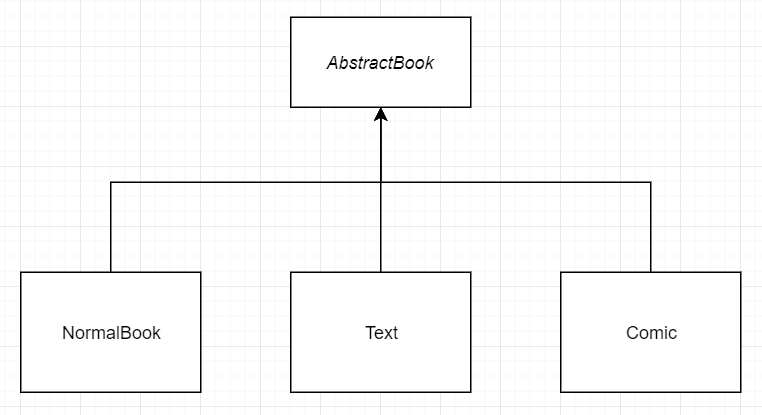
\includegraphics[width=0.5\textwidth]{images/hierarchy.png}
\end{center}

\begin{lstlisting}
class AbstractBook {
    string title, author;
    int length;
    protected:
        // Prevents assignment through base class pointers from compiling, but implementation still available to subclasses.
        AbstractBook &operator=(const AbstractBook &other);
    public:
        ...
        // Need at least one virtual method. If you don't have one, use the destructor.
        virtual ~AbstractBook() = 0; 
};

// Other classes are similar
class NormalBook: public AbstractBook {
    public:
        ...
        NormalBook &operator=(const NormalBook &other) {
            AbstractBook::operator=(other);
            return *this;
        }
        ~NormalBook() {}
};
\end{lstlisting}
\vspace{-0.25cm}
{\bf Note:} The virtual destructor {\bf must} be implemented, even though it is pure virtual.
\begin{lstlisting}
AbstractBook::~AbstractBook() {}
\end{lstlisting}

\newpage
\section{November 7, 2019}

\subsection{Templates}
\vspace{-0.1cm}
Consider:
\begin{lstlisting}
class List {
    struct Node;
    Node *theList;
    ...
};

struct List::Node {
    int data;
    Node *next;
};
\end{lstlisting}
\vspace{-0.25cm}
What if you want to store something else? We can write a new class -- or use a {\it template}.
\begin{lstlisting}
template <typename T> class List {
    struct Node {
        T data;
        Node *next;
    };
    Node *theList;
    public:
        class Iterator {
            Node *p;
            explicit Iterator(Node *p): p{p} {}
            public:
                T &operator*() { return p->data; }
                ...
        };
        T &ith(int i) { ... }
        void addToFront(T x) { ... };
        ...
};
\end{lstlisting}
\vspace{-0.25cm}
In the client, we can write:
\begin{lstlisting}
List<int> l1;
List<List <int>> l2;
l1.addToFront(3);
l2.addToFront(l1);
for(List<int>::Iterator it.l1.begin(); it != l1.end(); ++it) {
    cout << *it << endl;
}
for(auto n : l1) { ... }
\end{lstlisting}
The compiler specializes templates at the source code level, before compilation.

For templates, the entire implementation must go in the header.

\subsection{The Standard Template Library (STL)}
The STL contains a large number of useful templates.

For example, dynamic-length arrays: {\tt vector}.
\begin{lstlisting}
#include <vector>
using namespace std;

vector<int> v {4, 5}; // creates the vector 4 5
v.emplace_back(6); // 4 5 6
v.emplace_back(7); // 4 5 6 7
\end{lstlisting}
\vspace{-0.25cm}
Note: brace initialization is different from round brackets in this case.
\begin{lstlisting}
vector<int> v (4, 5); // produces 5 5 5 5
\end{lstlisting}
\vspace{-0.25cm}
Looping over vectors:
\begin{lstlisting}
for(int i = 0; i < v.size(); ++i) {
    cout << v[i] << endl;
}
for(vector<int>::iterator it = v.begin(); it != v.end(); ++it) {
    cout << *it << endl;
}
for(auto n : v) { ... }
\end{lstlisting}
\vspace{-0.25cm}
To iterate in reverse:
\begin{lstlisting}
for(vector<int>::reverse_iterator it = v.rbegin(); it != v.rend(); ++it) {
    ...
}
\end{lstlisting}
\vspace{-0.25cm}
{\tt rbegin} is one past the last element of the array, while {\tt rend} is one before the first element of the array.

To remove the last element:
\begin{lstlisting}
v.pop_back();
\end{lstlisting}
\vspace{-0.25cm}
Using iterators to remove items from inside a vector:
\begin{lstlisting}
auto it = v.erase(v.begin()); // erases first item
it = v.erase(v.begin() + 3); // erases 4th item
it = v.erase(it); // erases at current spot
v.erase(v.end() - 1); // erases last item
\end{lstlisting}
\vspace{-0.25cm}
{\tt erase} returns an iterator pointing to the first item after the erase.

{\tt v[i]} returns the $i$-th element of {\tt v}. This is unchecked -- if you go out of bounds, undefined behaviour occurs.

{\tt v.at(i)} is a checked version of {\tt v[i]}. What happens when you go out of bounds?

\subsection{Exceptions}
The problem: {\tt vector}'s code can detect the error, but it doesn't know what to do about it. The client can repond, but cannot detect the error.

The solution: Have functions return a status code, or set the global variable {\tt errno}. However, this style of programming encourages programmers to ignore error checks.

In C++, when an error condition arises, the function raises an {\it exception}. By default, execution stops. But we can write {\it handlers} to catch exceptions and deal with them.

{\tt vector<T>::at} throws {\tt std::out\_of\_range} when it fails. We can handle it as follows:
\begin{lstlisting}
#include <stdexcept>
...
try {
    cout << v.at(10000);
} catch(out_of_range r) {
    cerr << "Range error: " << r.what() << endl;
}
... // Execution resumes
\end{lstlisting}
\vspace{-0.25cm}
Now consider:
\begin{lstlisting}
void f() {
    throw out_of_range{"f"}; // constructor argument is what()
}
void g() { f(); }
void h() { g(); }
int main() {
    try {
        h();
    } catch(out_of_range) {
        ...
    }
}
\end{lstlisting}
\vspace{-0.25cm}
What happens?\vspace{-0.25cm}
\begin{itemize}[\label{}]
\item {\tt main} calls {\tt h}\vspace{-0.25cm}
\item {\tt h} calls {\tt g}\vspace{-0.25cm}
\item {\tt g} calls {\tt f}\vspace{-0.25cm}
\item {\tt f} raises {\tt out\_of\_range}
\end{itemize}
\vspace{-0.25cm}
Control goes back through the call chain ({\it unwinds} the stack) until a handler is found. This is all the way back to {\tt main} -- {\tt main} handles the exception.

If there is no matching handler in the entire call chain, the program terminates.

A handler might do part of the recovery job (i.e. execute some corrective code and throw another exception).
\begin{lstlisting}
try { ... }
catch(SomeErrorType s) {
    ... // corrective action
    throw SomeOtherError{ ... };
}
\end{lstlisting}
\vspace{-0.25cm}
It could rethrow the same exception:
\begin{lstlisting}
try { ... }
catch(SomeErrorType s) {
    ...
    throw; // as opposed to throw s
}
\end{lstlisting}
\vspace{-0.25cm}
Comparing {\tt throw} with {\tt throw s}:

{\tt throw}: The actual type of {\tt s} is retained.

{\tt throw s}: {\tt s} may be a subtype of {\tt SomeErrorType}, and thus throws an exception of type {\tt SomeErrorType}.

A handler can act as a catch-all. 
\begin{lstlisting}
try { ... }
catch(...) { // literally "..." in round brackets, catches all exceptions
    ...
}
\end{lstlisting}
\vspace{-0.25cm}
You can throw anything you want, not just objects.

\newpage
\section{November 12, 2019}

\subsection{Exceptions, Continued}
\emph{Never} let a destructor throw an exception. If this happens, the program will abort immediately. 

If you want a destructor to throw, you can tag it with {\tt noexcept(false)}, but this is not recommended. If a destructor is running during stack unwinding while dealing with another exception, and it throws, you now have \emph{two} active, unhandled exceptions. The program will abort immediately.

\subsection{Design Patterns, Continued}
Guiding principle:\vspace{-0.25cm}
\begin{itemize}
    \item Program to the interface, not the implementation.
    \item Abstract base classes define the interface. Work with base class pointers and call their methods.
    \item Concrete subclasses can be swapped in and out: abstraction over a variety of behaviours.
\end{itemize}
\vspace{-0.25cm}
For example, the Iterator pattern:
\begin{lstlisting}
class AbstractIterator {
    public:
        virtual int &operator*() = 0;
        virtual AbstractIterator &operator++() = 0;
        virtual bool operator!=(Abstract Iterator &other) = 0;
        virtual ~AbstractIterator();
};

class List {
    ...
    public:
        class Iterator : public AbstractIterator {
            ...
        };
};

class Set {
    ...
    public:
        class Iterator : public AbstractIterator {
            ...
        };
};
\end{lstlisting}
\vspace{-0.25cm}
Then, we can write code that operates over iterators. The following code works over {\tt List} and {\tt Sets}.
\begin{lstlisting}
void for_each(AbstractIterator &start, AbstractIterator &finish, int(*f)(int)) {
    while(start != finish) {
        f(*start);
        ++start;
    }
}
\end{lstlisting}

\subsection{Observer Pattern}
Consider a publish/subscribe model:\vspace{-0.25cm}
\begin{itemize}[\label{}]
    \item One class: publisher/subject -- generates data.
    \item One or more subscriber/observer class -- receive data and react to it.
\end{itemize}
\vspace{-0.25cm}
For example, the publisher could be spreadsheet cells, while the observers could be graphs. When cells change, the graphs update. 

There can be many different kinds of observer objects -- subject should not need to know all the details.

UML for the observer pattern:
\begin{center}
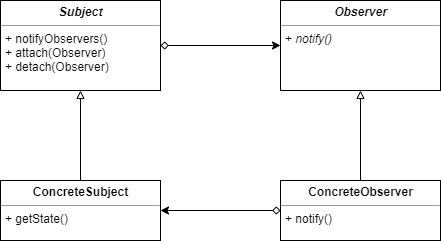
\includegraphics[width=0.75\textwidth]{images/observerUML.png}
\end{center}

Sequence of method calls:\vspace{-0.25cm}
\begin{enumerate}
    \item {\tt Subject}'s state is updated.
    \item {\tt Subject::notifyObservers()} -- calls each observer's {\tt notify}.
    \item Each observer calls {\tt ConcreteSubject::getState} to query \emph{the state}, and reacts accordingly.
\end{enumerate}
\vspace{-0.25cm}
For example: horse races. The subject publishes winners, and the observers are individual bettors: declare victory when their horse wins.
\begin{lstlisting}
// Subject and Observer classes are boilerplate code
class Subject {
    vector<Observer*> observers;
    public:
        void attach(Observer *ob) { observers.emplace_back(ob); }
        void detach(Observer *ob); // remove from observers
        void notifyObservers() { for(auto &ob : observers) ob->notify(); }
        virtual ~Subject() = 0;
};
Subject::~Subject() {}

class Observer {
    public:
        virtual void notify() = 0;
        virtual ~Observer() {}
};

// The following classes are specialized
class HorseRace : public Subject {
    ifstream in; // source of data
    string lastWinner;
    public:
        HorseRace(string source): in{source} {}
        bool runRace() {
            return in >> lastWinner;
        }
        string getState() { return lastWinner; }
};

class Bettor : public Observer {
    HorseRace *subject;
    string name, myHorse;
    public:
        Bettor( ... ): ... {
            subject->attach(this);
        }
        ~Bettor() { subject->detach(this); }
        void notify() {
            string winner = subject->getState();
            if(winner == myHorse) cout << "Win!" << endl;
            else cout << "Lose." << endl;
        }
};
\end{lstlisting}
\vspace{-0.25cm}
Now in main:
\begin{lstlisting}
HorseRace hr;
Bettor Larry {&hr, "Larry", "RunsLikeACow"};
... // other bettors
while(hr.runRace()) {
    hr.notifyObservers();
}
\end{lstlisting}

\subsection{Decorator Pattern}
The Decorator pattern is used if you want to enhance an object at runtime -- add functionality or features.

For example, consider a windowing system: start with a basic window. If you add enough text, add a scrollbar. If you press a certain key, add a menu. 

We want to choose these enhancements at runtime.

UML for decorator pattern:
\begin{center}
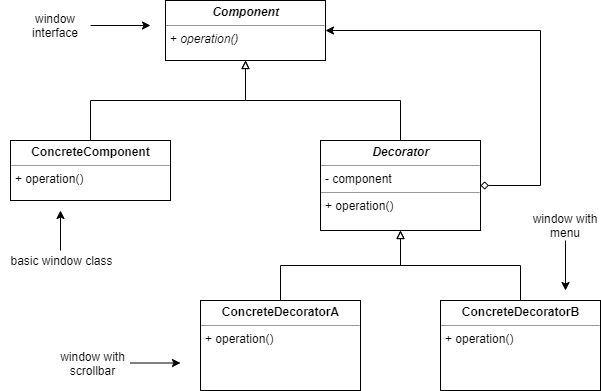
\includegraphics[width=0.9\textwidth]{images/decoratorUML.png}
\end{center}

{\tt Component}: Defines the interface -- operations your objects will provide.

{\tt ConcreteComponent}: Implements the interface.

{\tt Decorators}: All inherit from {\tt Decorator}, which inherits from {\tt Component}. Each decorator \emph{is} a {\tt Component} and \emph{has} a component.

For example, {\tt WindowWithScrollbar} is a kind of window and has a pointer to the underlying plain window.

{\tt WindowWithScrollbarAndMenu} \emph{is} a window and has a pointer to a {\tt WindowWithScrollbar}, which has a pointer to a window.

All inherit from {\tt WindowInterface}, so {\tt Window} methods can be used polymorphically on all of them.

For example, pizza:
\begin{center}
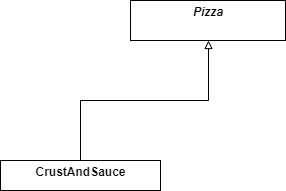
\includegraphics[width=0.4\textwidth]{images/pizza1.png}
\end{center}

Basic pizza is crust and sauce.
\begin{lstlisting}
class Pizza {
    public:
        virtual float price() const = 0;
        virtual string desc() const = 0;
        virtual ~Pizza() {}
};

class CrustAndSauce : public Pizza {
    public:
        float price() const override { return 5.99; }
        string desc() const override { return "pizza"; }
};
\end{lstlisting}
\vspace{-0.25cm}
Using the decorator pattern:
\begin{center}
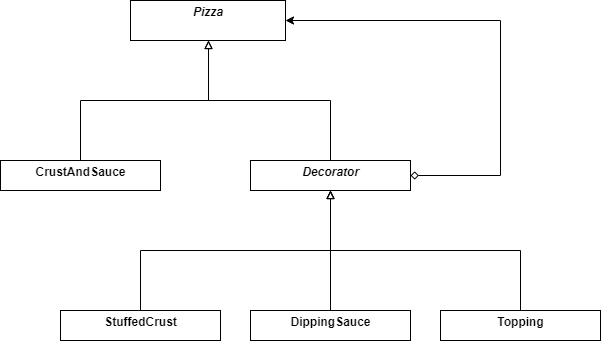
\includegraphics[width=0.7\textwidth]{images/pizza2.png}
\end{center}

\begin{lstlisting}
class Decorator : public Pizza {
    protected:
        Pizza *component;
    public:
        Decorator(Pizza *p): component{p} {}
        virtual ~Decorator() { delete component; }
};

class StuffedCrust : public Decorator {
    public:
        StuffedCrust(Pizza *p): Decorator{p} {}
        float price() const override { return component->price() + 2.69; }
        string desc() const override { return component->desc() + " with stuffed crust"; }
};
\end{lstlisting}

\newpage
\section{November 14, 2019}

\subsection{Factory Method Pattern}
Suppose we are making a video game with 2 kinds of enemies: turtles and bullets. The system randomly sends turtles and bullets, but bullets are more frequent in harder levels.
\begin{center}
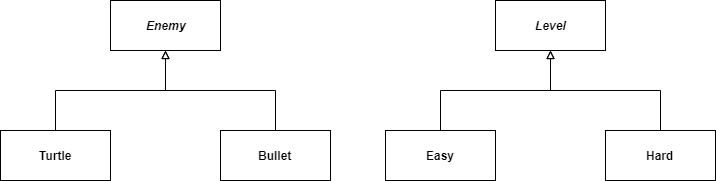
\includegraphics[width=0.9\textwidth]{images/game.png}
\end{center}
Instead, put a factory method in {\tt Level} that creates enemies.
\begin{lstlisting}
class Level {
    public:
        virtual Enemy *createEnemy() = 0;
};

class Easy : public Level {
    public:
        Enemy *createEnemy() override {
            // create mostly turtles
        }
};

class Hard : public Level {
    public:
        Enemy *createEnemy() override {
            // create mostly bullets
        }
};
\end{lstlisting}
\vspace{-0.25cm}
Then:
\begin{lstlisting}
Level *l = new Easy; // or Hard
Enemy *e = l->createEnemy();
\end{lstlisting}

\newpage
\subsection{Template Method Pattern}
Suppose we want subclasses to override superclass behaviour, but some aspects must stay the same.

For example, let's say there are red turtles and green turtles. 
\begin{lstlisting}
class Turtle {
    public:
        void draw() {
            drawHead();
            drawShell();
            drawFeet();
        }
    private:
        void drawHead() { ... }
        void drawFeet() { ... }
        virtual void drawShell() = 0;
};

class RedTurtle : public Turtle {
    void drawShell() override {
        // draw red shell
    }
};

class GreenTurtle : public Turtle {
    void drawShell() override {
        // draw green shell
    }
};
\end{lstlisting}
\vspace{-0.25cm}
Subclasses cannot access the private methods of the superclass, but they may override them.

In the above example, subclasses cannot change the way a turtle is drawn (head, shell, feet), but can change the way the shell is drawn.

Generalization: the non-virtual interface (NVI) idiom.

A public virtual method is really two things:\vspace{-0.25cm}
\begin{itemize}
    \item public: An interface to the client. It indicates provided behaviour with pre- and post-conditions.
    \item virtual: An interface to subclasses. A "hook" to insert specialized behaviour.
\end{itemize}
\vspace{-0.25cm}
These are conflicting goals.

NVI says that:\vspace{-0.25cm}
\begin{itemize}
    \item all public methods should be non-virtual
    \item all virtual methods should be private (or at least protected), except the destructor
\end{itemize}
\vspace{-0.25cm}
The following example does not conform to NVI:
\begin{lstlisting}
class DigitalMedia {
    public:
        virtual void play() = 0;
};
\end{lstlisting}
\vspace{-0.25cm}
We can modify it so that it does:
\begin{lstlisting}
class DigitalMedia {
    public:
        void play() {
            doPlay();
        }
    private:
        virtual void doPlay() = 0;
};
\end{lstlisting}
\vspace{-0.25cm}
This code does the same thing, except we have more control now. We can also add before and after code within {\tt play()} (e.g. copyright check, updating play count).

This generalizes the template method pattern: it puts every virtual method inside a template method.

\subsection{STL Maps For Creating Dictionaries}
Consider "arrays" that map strings to integers.
\begin{lstlisting}
#include <map>
using namespace std;
map<string, int> m;
m["abc"] = 1;
m["def"] = 4;
cout << m["ghi"] << m["def"]; // 04
\end{lstlisting}
\vspace{-0.25cm}
If the key is not present, it is inserted and the value is default-constructed (in this case, 0).
\begin{lstlisting}
m.erase("abc");
if(m.count("def")) ... // 0 means not found, 1 means found
\end{lstlisting}
\vspace{-0.25cm}
Iterating over a map: sorted key order. 
\begin{lstlisting}
for(auto &p : m) {
    cout << p.first << ' ' << p.second << endl;
}
\end{lstlisting}
\vspace{-0.25cm}
{\tt p}'s type is {\tt std::pair<string, int>} from {\tt <utility>}. Also note that {\tt first} and {\tt second} are public fields, which makes sense since it is not meant to be an abstraction.

\subsection{Visitor Pattern}
The visitor pattern is used for implementing {\bf double dispatch}. 

Virtual methods are chosen based on the actual type (at runtime) of the receiving object. What if you want to choose based on two objects?

Consider once again the video game example: striking enemies with weapons.
\begin{center}
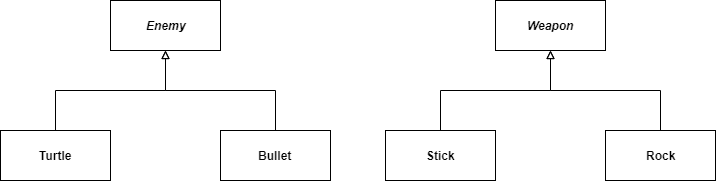
\includegraphics[width=0.9\textwidth]{images/game2.png}
\end{center}
We would like to write something like:
\begin{lstlisting}
virtual void(Enemy, Weapon)::strike();
\end{lstlisting}
\vspace{-0.25cm}
However, this is not legal C++.

If {\tt strike} is a method of {\tt Enemy}, we choose based on an enemy, but not a weapon.

If {\tt strike} is a method of {\tt Weapon}, we choose based on a weapon, but not an enemy.

The trick to get dispatch on both (double dispatch): combine overriding and overloading.
\begin{lstlisting}
class Enemy {
    public:
        virtual void beStruckBy(Weapon &w) = 0;
};

class Turtle : public Enemy {
    public:
        void beStruckBy(Weapon &w) override { w.strike(*this); }
};

class Bullet : public Enemy {
    public:
        void beStruckBy(Weapon &w) override { w.strike(*this); }
};
\end{lstlisting}
\vspace{-0.25cm}
They appear the same, but in the case of {\tt Turtle}, {\tt *this} is of type {\tt Turtle\&}, while in {\tt Bullet}, {\tt *this} is of type {\tt Bullet\&}. These are two different overloads of {\tt strike}.
\newpage
\begin{lstlisting}
class Weapon {
    public:
        virtual void strike(Turtle &t) = 0;
        virtual void strike(Bullet &b) = 0;
};

class Stick : public Weapon {
    public:
        void strike(Turtle &t) override { /* strike turtle with stick */ }
        void strike(Bullet &b) override { /* strike bullet with stick */ }
};

class Rock : public Weapon {
    public:
        void strike(Turtle &t) override { /* strike turtle with rock */ }
        void strike(Bullet &b) override { /* strike bullet with rock */ }
};
\end{lstlisting}
\vspace{-0.25cm}
Now, consider:
\begin{lstlisting}
Enemy *e = new Bullet; // don't know type of enemy, assume Bullet
Weapon *w = new Rock; // don't know type of weapon, assume Rock
e->beStruckBy(w);
\end{lstlisting}
\vspace{-0.25cm}
What happens?

{\tt Bullet::beStruckBy} runs (virtual method) \\
It calls {\tt Weapon::strike}, {\tt *this} is of type {\tt Bullet} \\
{\tt Bullet} version of {\tt strike} is chosen at compile-time \\
Virtual method {\tt strike} on {\tt Weapon} resolves to {\tt Rock::strike(Bullet \&)}

\newpage
\section{November 19, 2019}

\subsection{Visitor Pattern, Continued}
The visitor pattern can be used to add functionality to existing classes, without changing or recompiling the classes themselves.

For example, consider adding a visitor to the {\tt Book} hierarchy.
\begin{lstlisting}
class Book {
public:
    virtual void accept(BookVisitor &v) { v.visit(*this); }
    ...
};

class Text : public Book {
public:
    void accept(BookVisitor &v) { v.visit(*this); }
};

class BookVisitor {
public:
    virtual void visit(Book &b) = 0;
    virtual void visit(Text &t) = 0;
    virtual void visit(Comic &c) = 0;
};
\end{lstlisting}
\vspace{-0.25cm}
We claim that this is the same as the striking enemies with weapons example above. If we replace {\tt Book} with {\tt Enemy}, {\tt accept} with {\tt beStruckBy}, and {\tt Visitor} with {\tt Weapon}, they are indeed the same.

{\bf Application:} Track how many of each type of {\tt Book} we have: \vspace{-0.5cm}
\begin{itemize}[label={}]
\item {\tt Book}: by author\vspace{-0.25cm}
\item {\tt Text}: by topic\vspace{-0.25cm}
\item {\tt Comic}: by hero\vspace{-0.25cm}
\end{itemize}
\vspace{-0.25cm}
We can use a {\tt map<string, int>}. We could write a virtual {\tt updateMap} method, or write a visitor.
\begin{lstlisting}
struct Catalogue : public BookVisitor {
    map<string, int> theCat;
    void visit(Book &b) override { ++theCat[b.getAuthor()]; }
    void visit(Text &t) override { ++theCat[t.getTopic()]; }
    void visit(Comic &c) override { ++theCat[c.getHero()]; }
};
\end{lstlisting}

\newpage
\subsection{Compilation Dependencies}
When does a file \emph{need} to include another file?

{\bf Remark:} A long sequence of includes in the beginning of compile errors is an indicator that there is a cycle of includes.

Consider:
\begin{lstlisting}
// a.h
class A { ... }; 
\end{lstlisting}
\vspace{-0.25cm}
The following are modules that have {\tt A} in them:
\begin{lstlisting}
// b.h
#include "a.h"
class B : public A {
    ...
};

// c.h
#include "a.h"
class C {
    A a;
}; 

// d.h
class A;
class D {
    A *pa;
};

// e.h
class A;
class E {
    A f(A a);
};

// f.h
#include "a.h"
class F {
    A f(A a) { a.g() }
};
\end{lstlisting}
\vspace{-0.25cm}
For {\tt B} and {\tt C}, we need to know the size of {\tt A}, so we need to include {\tt a.h}. 

For {\tt D} and {\tt E}, there is no compilation dependency: they just need to know that {\tt A} exists. In the case of {\tt D}, all pointers are the same size. In the case of {\tt E}, we don't need to know anything about {\tt A}.

For {\tt F}, we need details about {\tt A}, so we need an include.

If the code doesn't need an include, don't create a needless compilation dependency by including unnecessarily.

When {\tt A} changes, only {\tt A}, {\tt B}, {\tt C}, and {\tt F} need recompilation.

In the \emph{implementations} of {\tt D} and {\tt E}:
\begin{lstlisting}
// d.cc
#include "a.h"
void D::f() {
    pa->something();
}
\end{lstlisting}
\vspace{-0.25cm}
Do the include in the {\tt .cc} file instead of the {\tt .h} file (where possible).

\subsection{Bridge Pattern}
Consider the {\tt XWindow} class:
\begin{lstlisting}
class XWindow {
    Display *d;
    Window w;
    int s;
    GC gc;
    unsigned long colours[10];
public:
    ...
};
\end{lstlisting}
\vspace{-0.25cm}
What if we need to add or change a private member? All clients must recompile. It would be better to hide these details away.

{\bf Solution:} {\tt pImpl} idiom ("pointer to implementation")

Create a second class {\tt XWindowImpl}:
\begin{lstlisting}
// XWindowImpl.h
#include <X11/Xlib.h>
struct XWindowImpl {
    Display *d;
    Window w;
    int s;
    GC gc;
    unsigned long colours[10];
};

// Window.h
class XWindowImpl;
class XWindow {
    XWindowImpl *pImpl;
public:
    ... // no change
};
\end{lstlisting}
\vspace{-0.25cm}
Notes on the {\tt Window.h} class:\vspace{-0.25cm}
\begin{itemize}
\item There is no need to include {\tt Xlib.h}.
\item We forward declare the {\tt Impl} class ({\tt class XWindowImpl;}).
\item There is no compilation dependecy on {\tt XWindowImpl.h}. 
\item Clients also don't depend on {\tt XWindowImpl.h}.
\end{itemize}
\begin{lstlisting}
// Window.cc
#include "Window.h"
#include "XWindowImpl.h"
XWindow::XWindow( ... ): pImpl{new XWindowImpl} {}
XWindow::~XWindow() { delete pImpl; }
\end{lstlisting}
\vspace{-0.25cm}
For other methods, replace fields {\tt d}, {\tt w}, {\tt s}, {\tt gc}, {\tt colours} with {\tt pImpl->d}, {\tt pImpl->w}, {\tt pImpl->s}, {\tt pImpl->gc}, and {\tt pImpl->colours}.

When changing private fields, we only need to recompile {\tt Window.cc} and relink.

Generalization: What if there are several possible window implementations, say {\tt XWindow} and {\tt YWindow}. 

Then make {\tt Impl} struct a superclass.
\begin{center}
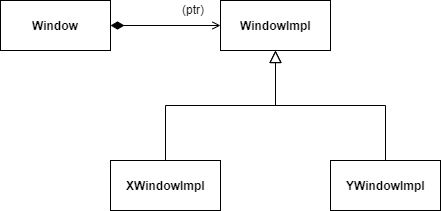
\includegraphics[width=0.7\textwidth]{images/pimpl.png}
\end{center}

The {\tt pImpl} idiom and hierarchy of implementations is called the \emph{bridge pattern}.

\subsection{Measures of Design Quality}
{\bf Coupling:} How much distinct modules depend on each other.

Low coupling:\vspace{-0.25cm}
\begin{itemize}
\item Communicate via function calls with basic parameters and results.
\item Modules pass arrays and structs back and forth.
\item Modules affect each other's control flow.
\end{itemize}
\vspace{-0.25cm} High coupling: \vspace{-0.25cm}
\begin{itemize}
\item Modules have access to each other's implementation (friends).
\end{itemize}
{\bf Cohesion:} How closely elements of a module are related to each other.

Low cohesion:\vspace{-0.25cm}
\begin{itemize}
\item Arbitrary grouping of unrelated elements (e.g. {\tt <utility>}). 
\item Slightly more cohesive: elements share a common theme, otherwise unrelated, maybe share some base code (e.g. {\tt <algorithm>}).
\item Elements manipulate state over the lifetime of an object (e.g. open/read/close files).
\item Elements pass data to each other.
\end{itemize}
\vspace{-0.25cm} High cohesion: \vspace{-0.25cm}
\begin{itemize}
\item Elements cooperate to perform exactly one task.
\end{itemize}
\vspace{-0.25cm}
Low cohesion results in poorly organized code. 

The goal is to achieve low coupling and high cohesion.

\newpage
\section{November 21, 2019}

\subsection{Decoupling the Interface (MVC)}
Your primary program class should not be printing things.
\begin{lstlisting}
class Chessboard {
    ...
    cout << "Your move" << endl;
};
\end{lstlisting}
\vspace{-0.25cm}
This is bad design: it inhibits code reuse. 

What if you want to reuse {\tt Chessboard}, but not have it communicate via stdout?

We could give the class stream objects, where it can send its input/output.
\begin{lstlisting}
class Chessboard {
    istream &in;
    ostream &out;
    ...
    out << "Your move" << endl;
};
\end{lstlisting}
\vspace{-0.25cm}
This is better, but what if we don't want to use streams at all?

{\tt Chessboard} should not be doing any communication at all.

{\bf Single Responsibility Principle:} "A class should have only one reason to change."

The game state and communication are \emph{two} reasons.

A better option: communicate with the chessboard via parameters or results. Confine user communication to outside the game class.

{\tt main} should not be communicating -- it is hard to reuse code if it is in {\tt main}. 

There should be a class to manage interaction, separate from the state class.

{\bf Architecture: Model-View-Controller (MVC)}

Separate the distinct notions of the data ("model"), the presentation of the data ("view"), and the control or manipulation of the data ("controller").
\begin{center}
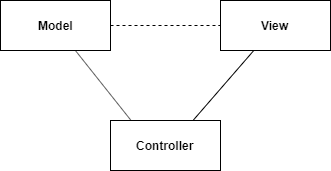
\includegraphics[width=0.4\textwidth]{images/mvc.png}
\end{center}
The model can have multiple views (e.g. text/graphics). It doesn't need to know their details. This is a classic Observer pattern (or could communicate through controller).

The controller mediates control flow between model and view. It might handle input (or could be the view).

This decouples presentation and control, and as a result, promotes reuse.

\subsection{Exception Safety}
Consider:
\begin{lstlisting}
void f() {
    MyClass mc;
    MyClass *p = new MyClass;
    g();
    delete p;
}
\end{lstlisting}
\vspace{-0.25cm}
There are no leaks -- but what if {\tt g} throws?

During stack unwinding, all stack-allocated data is cleaned up. The destructors run, and memory is reclaimed.

However, heap-allocated objects are not destroyed. Therefore, if {\tt g} throws, {\tt *p} is leaked ({\tt mc} is not).
\begin{lstlisting}
void f() {
    MyClass mc;
    MyClass *p = new myClass;
    try {
        g();
    } catch(...) {
        delete p;
        throw;
    }
    delete p;
}
\end{lstlisting}
\vspace{-0.25cm}
This works: but there is duplication of code. How else can we guarantee that something (e.g. {\tt delete p}) will happen no matter how we exit {\tt f} (normal or exception)?

In some languages, "finally" clauses guarantee certain final actions -- C++ is not one of them.

The only thing we can count on in C++: destructors for stack-allocated data will run.

Therefore, use stack-allocated data with destructors as much as possible: use the guarantee to your advantage.

{\bf C++ idiom: Resource Acquisition Is Initialization (RAII)}

Every resource should be wrapped in a stack-allocated object whose job is to delete it. 

For example, files:
\begin{lstlisting}
void foo() {
    ifstream f{"file"};
    ...
}
\end{lstlisting}
\vspace{-0.25cm}
Acquiring the resource ({\tt "file"}) is initializing the object.

The file is guaranteed to be released when {\tt f} is popped from the stack ({\tt f}'s destructor runs).

This can be done with dynamic memory:
\begin{lstlisting}
#include <memory>
class std::unique_ptr<T>
\end{lstlisting}
\vspace{-0.25cm}
This takes a {\tt T*} in the constructor. The destructor will delete the pointer. In between, we can deference, just like a pointer.
\begin{lstlisting}
void f() {
    MyClass mc;
    std::unique_ptr<MyClass> p{new MyClass};
    g();
}
\end{lstlisting}
\vspace{-0.25cm}
Now, we are guaranteed to have no leaks.

We can phrase the above slightly differently:
\begin{lstlisting}
void f() {
    MyClass mc;
    auto p = make_unique<MyClass>(); // constructor arguments in parenthesis
    g();
}
\end{lstlisting}
\vspace{-0.25cm}
Difficulty:
\begin{lstlisting}
unique_ptr<C> p{new C{...}};
unique_ptr<C> q = p;
\end{lstlisting}
\vspace{-0.25cm}
What happens when a {\tt unique\_ptr} is copied? We don't want to delete the same pointer twice (double free). 

Instead: copying is disabled for {\tt unique\_ptr} -- they can only be moved. 

However, we can have one {\tt unique\_ptr} and many regular pointers to an object, and we can think of this as ownership of the resource.

\newpage
A simple implementation of {\tt unique\_ptr} (repo):
\begin{lstlisting}
template<typename T> class unique_ptr {
    T *ptr;
public:
    unique_ptr(T *p): ptr{p} {}
    ~unique_ptr() { delete ptr; }
    unique_ptr(const unique_ptr &other) = delete;
    unique_ptr &operator=(const unique_ptr &other) = delete;
    unique_ptr(unique_ptr &&other): ptr{other.ptr} {
        other.ptr = nullptr;
    }
    unique_ptr &operator=(unique_ptr &&other) {
        std::swap(ptr, other.ptr);
        return *this;
    }
    T &operator*() { return *ptr; }
}
\end{lstlisting}
\vspace{-0.25cm}
{\tt unique\_ptr} also has a method called {\tt get}:
\begin{lstlisting}
T *q = p.get();
\end{lstlisting}
\vspace{-0.25cm}
This can also be done:
\begin{lstlisting}
T *q = &*p;
\end{lstlisting}
\vspace{-0.25cm}
{\bf Copying Pointers}

First, we need to answer the question of ownershiip.

Who will own the resource? Who will have responsibility for freeing it?

That pointer should be a {\tt unique\_ptr} -- all other pointers can be raw pointers (can fetch the underlying raw pointer with {\tt p.get()}).

If there is true shared ownership (i.e. any of several pointers might need to free the resource), use {\tt std::shared\_ptr}.
\begin{lstlisting}
void f() {
    auto p1 = std::make_shared<MyClass>();
    if( ... ) {
        auto p2 = p1;
    } // p2 popped, pointer not deleted
} // p1 popped, pointer is deleted
\end{lstlisting}
\vspace{-1.5ex}
Shared pointers maintain a \emph{reference count}, the count of all {\tt shared\_ptr}s pointing at the same object. Memory is freed when the number of {\tt shared\_ptr}s pointing to it is about to hit 0.

\newpage
\section{November 26, 2019}
\subsection{Back to Exception Safety}
Three levels of exception safety for a function {\tt f}:\vspace{-1.5ex}
\begin{enumerate}
    \item {\bf Basic guarantee:} If an exception occurs, the program will be left in some valid state (no leaks, no corrupted data structures, and invariants are maintained).
    \item {\bf Strong guarantee:} If an exception is raised while executing {\tt f}, the state of the program will be as it was before {\tt f} was called.
    \item {\bf No-throw guarantee:} The function {\tt f} will never throw or propogate an exception, and will always accomplish its task.
\end{enumerate}
\vspace{-1.5ex}
For example:
\begin{lstlisting}
class A { ... };
class B { ... };
class C {
    A a;
    B b;
public:
    void f() {
        a.g(); // may throw (strong guarantee)
        b.h(); // may throw (strong guarantee)
    }
};
\end{lstlisting}
\vspace{-1.5ex}
Is {\tt C::f} exception safe?

If {\tt a.g()} throws, nothing has happened yet, so there are no problems.

If {\tt b.h()} throws, the effects of {\tt a.g()} must be undone to offer the strong guarantee. This is very hard or impossible to do if {\tt a.g()} has non-local side effects.

So {\tt C::f} is not exception safe. 

If {\tt A::g} and {\tt B::h} do not have non-local side effects, we can use copy-and-swap.
\begin{lstlisting}
class C {
    ...
    void f() {
        // If the first four lines throw, original is intact
        A atemp = a;
        B btemp = b;
        atemp.g();
        btemp.h();
        // What happens if copy assignment throws?
        a = atemp;
        b = btemp;
    }
};
\end{lstlisting}
\vspace{-1.5ex}
It would be better if the "swap" part was no-throw. Copying pointers cannot throw.

Solution: Use the {\tt pImpl} idiom.
\begin{lstlisting}
struct CImpl {
    A a;
    B b;
};

class C {
    unique_ptr<CImpl> pImpl;
    ...
    void f() {
        auto temp = make_unique<CImpl>(*pImpl);
        temp->a.g();
        temp->b.h();
        std::swap(pImpl, temp); // no throw
    }
};
\end{lstlisting}
\vspace{-1.5ex}
Now, {\tt C::f} has strong guarantee.

\subsection{Exception Safety and the STL: Vectors}
Vectors encapsulate a heap-allocated array. They follow RAII: when a stack-allocated vector goes out of scope, the internal heap-allocated array is freed.
\begin{lstlisting}
void f() {
    vector<MyClass> v;
    ...
}
\end{lstlisting}
\vspace{-1.5ex}
When {\tt v} goes out of scope, the array is freed, and the {\tt MyClass} destructor runs on all objects in the vector.

However:
\begin{lstlisting}
void g() {
    vector<MyClass*> v;
    ...
}
\end{lstlisting}
\vspace{-1.5ex}
The array is freed. Pointers don't have destructors, so any objects pointed at by the pointers are not deleted.

{\tt v} doesn't know whether the pointers in the array \emph{own} the objects they point at.

Now consider:
\begin{lstlisting}
void h() {
    vector<unique_ptr<MyClass>> v;
    ...
}
\end{lstlisting}
\vspace{-1.5ex}
The array is freed, the {\tt unique\_ptr} destructor runs, so the objects \emph{are} deleted. We don't have to do any explicit deallocation.

Now, consider {\tt vector<T>::emplace\_back}, which offers the strong guarantee. This is because if the array is full (i.e. {\tt size == cap}):\vspace{-1.5ex}
\begin{itemize}
    \item New array is allocated.
    \item Copy objects over (copy constructor) -- if a copy constructor throws, destroy the new array, and the old array is still intact.
    \item Delete old array (no-throw).
\end{itemize}
\vspace{-1.5ex}
But copying is expensive and the old data will be thrown away. Wouldn't moving the objects be more efficient? 

The old array is no longer intact if the move constructor throws, so we cannot offer the strong guarantee.

If the move constructor offers the no-throw guarantee, then {\tt emplace\_back} will use the move constructor. Otherwise, it will use the copy constructor, which will be slower.

So, move operations should offer the no-throw guarantee, and you should indicate that they do.
\begin{lstlisting}
class MyClass {
public:
    ...
    MyClass(MyClass &&other) noexcept { ... }
    MyClass &operator=(MyClass &&other) noexcept { ... }
};
\end{lstlisting}
\vspace{-1.5ex}
If you know a function will never throw or propagate an exception, declare it {\tt noexcept}, which facilitates optimization. 

At the minimum, moves and swaps should be {\tt noexcept}.

\newpage
\section{November 28, 2019}
\subsection{Casting}
In C:
\begin{lstlisting}
struct Node n;
int *ip = (int*) &n; 
\end{lstlisting}\vspace{-1.5ex}
The above is a cast: it forces C to treat a {\tt Node*} as an {\tt int*}.

C-style casts should be avoided in C++. If you must cast, use a C++-style cast. 

There are four kinds:\vspace{-1.5ex}
\begin{itemize}
\item {\tt static\_cast} -- "sensible casts" 

For example, {\tt double} to {\tt int}:
\begin{lstlisting}
double d;
void f(int x);
void f(double x);
f(static_cast<int>(d));
\end{lstlisting}
\vspace{-1ex}
Superclass pointer to subclass pointer:
\begin{lstlisting}
Book *b = new Text{ ... };
Text *t = static_cast<Text*>(b); // t->getTopic() valid
\end{lstlisting}
\vspace{-1ex}
{\bf Note:} You are taking responsibility that {\tt b} actually points at a {\tt Text}. If this is wrong, it results in undefined behaviour.

\item {\tt reinterpret\_cast} -- unsafe, implementation-specific, "weird" casts
\begin{lstlisting}
Student s;
Turtle *t = reinterpret_cast<Turtle*>(&s);
\end{lstlisting}\vspace{-1ex}

\item {\tt const\_cast} -- for converting between const and non-const

This is the only C++ cast that can "cast away const".
\begin{lstlisting}
void g(int *p); // know that g doesn't modify p
void f(const int *p) {
    ...
    g(const_cast<int*>(p));
    ...
}
\end{lstlisting}\vspace{-1ex}

\item {\tt dynamic\_cast} -- unsure if it is safe to convert, better to do a tentative cast and see if it works
\begin{lstlisting}
Book *pb;
Text *pt = dynamic_cst<Text*>(pb);
\end{lstlisting}\vspace{-1ex}
If the cast works ({\tt *pb} really is a {\tt Text} or a subclass of {\tt Text}), then {\tt pt} points at the object. Otherwise, {\tt pt} will be {\tt nullptr}.
\begin{lstlisting}
if(pt) cout << pt->getTopic();
else cout << "Not a text";
\end{lstlisting}

\end{itemize}\vspace{-1.5ex}
But these are all operations on raw pointers. Can we do this with smart pointers?

Yes: {\tt static\_pointer\_cast}, {\tt const\_pointer\_cast}, and {\tt dynamic\_pointer\_cast} all cast {\tt shared\_ptr}s to {\tt shared\_ptr}s.

We can use dynamic casting to make decisions based on an objects run-time type information (RTTI).
\begin{lstlisting}
void whatIsIt(shared_ptr<Book> b) {
    if(dynamic_pointer_cast<Comic>(b)) cout << "Comic";
    else if(dynamic_pointer_cast<Text>(b)) cout << "Text";
    else cout << "Normal book";
}
\end{lstlisting}\vspace{-1.5ex}
However, this code is tightly coupled to the {\tt Book} hierarchy, and may indicate bad design. 

Better options: use virtual methods or visitor pattern (if possible).

Dynamic casting also works with references:
\begin{lstlisting}
Text t { ... };
Book &b = t;
Text &t2 = dynamic_cast<Text&>(b);
\end{lstlisting}\vspace{-1.5ex}
If {\tt b} points to a {\tt Text}, then {\tt t2} is a reference to the same {\tt Text}.

If not, the exception {\tt bad\_cast} is raised (no such thing as a null reference).

{\bf Note:} Dynamic casting only works on classes with at least one virtual method.

With dynamic reference casting, we can now solve the polymorphic assignment problem.
\begin{lstlisting}
Text &Text::operator=(const Book &other) { // virtual 
    const Text &textOther = dynamic_cast<const Text&>(other);
    if(this == &textOther) return *this;
    Book::operator=(other);
    topic = textOther.topic;
    return *this;
}
\end{lstlisting}\vspace{-1.5ex}
If {\tt other} is not a text, then dynamic casting throws, and none of the operations after occur. 

\newpage
\subsection{How Virtual Methods Work}
Consider the following two classes:
\begin{lstlisting}
class Vec {
    int x, y;
public:
    void f() { ... }
};

class Vec2  {
    int x, y;
public:
    virtual void f() { ... }
};
\end{lstlisting}\vspace{-1.5ex}
What is the difference?
\begin{lstlisting}
Vec v {1, 2};
Vec2 w {1, 2};
\end{lstlisting}\vspace{-1.5ex}
Do they look the same in memory?
\begin{lstlisting}
cout << sizeof(v) << ' ' << sizeof(w); // 8 16
\end{lstlisting}\vspace{-1.5ex}
First, note that 8 is the space for 2 ints, and there is no space for the {\tt f} method.

The compiler turns methods into ordinary functions and stores them separately from objects.

Recall that if a method is virtual, the choice of which version to run is based on the type of the actual object, which the compiler can't know at compile-time.

The correct method must be chosen at run-time.

For each class with virtual methods, the compiler creates a table of functions pointers (the vtable). 
\begin{lstlisting}
class C {
    int x, y;
    virtual void f();
    virtual void g();
    void h();
    virtual ~C();
};
\end{lstlisting}\vspace{-1.5ex}
The vtable then looks like
\begin{table}[h]
\centering
\begin{tabular}{|l|}
\hline
{\tt C}  \\ \hline
{\tt f}  \\ \hline
{\tt g}  \\ \hline
\texttt{\~{}C} \\
\hline
\end{tabular}
\end{table}

with each of the entries pointing to the actual code {\tt C::f}, {\tt C::g}, and {\tt C::\~{}C}. 

{\tt C}'s objects have an extra pointer (the vptr) that points to {\tt C}'s vtable.

What occurs when a virtual method is called:\vspace{-1.5ex}
\begin{itemize}
    \item Follow vptr to vtable.
    \item Fetch the pointer to the action method from table.
    \item Follow the function pointer and call the function.
\end{itemize}\vspace{-1.5ex}
All of these occur at run-time.

Virtual function calls incur a small overhead cost. Also, declaring at least one virtual method adds a pointer to the object, a vptr. Thus, classes with no virtual methods produce smaller objects than if some functions were virtual.

\newpage
\section{December 3, 2019}

\subsection{How Objects are Laid Out}
Concretely, how is an object laid out? This is compiler dependent. 

In g++:
\begin{lstlisting}
class A {
    int a, c;
    virtual void f();
};

class B: public A {
    int b, d;
};
\end{lstlisting}\vspace{-1.5ex}

\begin{table}[h]
\centering
\begin{tabular}{|c|cl|c|}
\cline{1-1} \cline{4-4}
vptr    &  &  & vptr    \\ \cline{1-1} \cline{4-4} 
{\tt a} &  &  & {\tt a} \\ \cline{1-1} \cline{4-4} 
{\tt c} &  &  & {\tt c} \\ \cline{1-1} \cline{4-4} 
        &  &  & {\tt b} \\ \cline{1-1} \cline{4-4} 
        &  &  & {\tt d} \\ \cline{1-1} \cline{4-4} 
\end{tabular}
\end{table}

This is better so that a pointer to {\tt B} looks like a pointer to {\tt A} if you ignore the last two fields. Also, you will always know where the vptr is (always first).

\subsection{Multiple Inheritance}
A class can inherit from more than one class.
\begin{lstlisting}
class A {
public:
    int a;
};

class B {
public:
    int b;
};

class C: public A, public B {
    row f() {
        cout << a << ' ' << b;
    }
};
\end{lstlisting}\vspace{-1.5ex}
{\bf Challenges}

Suppose {\tt b} and {\tt c} inherit from {\tt A}.
\begin{lstlisting}
class D: public B, public C {
public:
    int d;
};
\end{lstlisting}\vspace{-1.5ex}
If {\tt B} and {\tt c} from {\tt A}, should there be one {\tt A} prt of {\tt D}< or two (default)?

Should {\tt B::a} and {\tt C::a} be the same or different?

Consider the "deadly diamond".
%% 

Make {\tt A} a virtual base class -- virtual inheritance.
\begin{lstlisting}
class B: virtual public A { ... };
class C: virtual public A { ... };
\end{lstlisting}\vspace{-1.5ex}
How will this be laid out?

vptr\\
{\tt A} fields\\
{\tt B} fields\\
{\tt C} fields\\
{\tt D} fields\\

g++: 

vptr\\
{\tt B} fields\\
vptr <-- {\tt C*}\\
{\tt C} fields\\
{\tt D} fields\\
vptr <-- {\tt A*}\\
{\tt A} fields

{\tt B} needs to be laid out so that we can find its {\tt A} part, but these diagrams show that the distance to the {\tt A} part isn't necessarily there.

{\sc Solution:} The location of the base class is stored in the vtables.

The diagram doesn't look like all of {\tt A}, {\tt B}, {\tt C}, {\tt D} simultaneously, but slices of it look like {\tt A}, {\tt B}, {\tt C}, {\tt D}. 

Pointer assignment among {\tt A}, {\tt B}, {\tt C}, {\tt D} changes the address stored in the pointer.
\begin{lstlisting}
D *d = ...;
A *a = d; // changes its address to point at the A part
\end{lstlisting}\vspace{-1.5ex}
Note: {\tt static\_cast}, {\tt dynamic\_cast} will do this, while {\tt reinterpret\_cast} will not.

\subsection{Template Functions}
Consider:
\begin{lstlisting}
template<typename T> T min(T x, T y) {
    return x < y ? x : y;
}

int f() {
    int x = 1, y = 2;
    int z = min(x, y); // don't have to say min<int>
}
\end{lstlisting}\vspace{-1.5ex}
C++ can infer that {\tt T} is an {\tt int} from the types of {\tt x} and {\tt y}. This applies to template functions only. 

If C++ cannot determine {\tt T}, you can always tell it explicitly: {\tt z = min<int>(x, y);}.
\begin{lstlisting}
char w = min('a', 'c'); // T = char
auto f = min(1.0, 3.0); // T = double
\end{lstlisting}\vspace{-1.5ex}
For what types {\tt T} can {\tt min} be used? Any type for which {\tt operator<} is defined.

Recall:
\begin{lstlisting}
void for_each(AbstractIterator start, AbstractIterator finish, int(*f)(int)) {
    while(start != finish) {
        f(*start);
        ++start;
    }
}
\end{lstlisting}\vspace{-1.5ex}
This works as long as {\tt AbstractIterator} supports {\tt !=}, {\tt *}, {\tt ++}. Also, {\tt f} can be called as a function.
\begin{lstlisting}
template<typename Iter, typename Fn>;
void for_each(Iter start, Iter finish, Fn f) {
    while(start != finish) {
        f(*start);
        ++start;
    }
}
\end{lstlisting}\vspace{-1.5ex}
Now, for example, we can write
\begin{lstlisting}
void f(int n) { cout << n << endl; }
int a[] = {1, 2, 3, 4, 5};
for_each(a, a + 5, f); // prints the array
\end{lstlisting}\vspace{-1.5ex}

{\bf C++ STL Library {\tt <algorithm>}}
\begin{lstlisting}
template<typename InIter, typename OutIter>
OutIter copy(InIter first, InIter last, OutIter result) {
    /* Copies one container range [first, last) to another,
       starting at result. 
       Note: does not allocate new memory. */
}
\end{lstlisting}\vspace{-1.5ex}
For example:
\begin{lstlisting}
vector<int> v {1, 2, 3, 4, 5, 6, 7};
vector<int> w(4); // space for 4 ints
copy(v.begin() + 1, v.begin() + 5, w.begin()); // w = {2, 3, 4, 5}
\end{lstlisting}
\end{document}